\cotefile{143}
\scanpage{1}
IMAG

INSTITUT MONTPELLIERAIN

ALEXANDER GROTHENDIECK

\figure{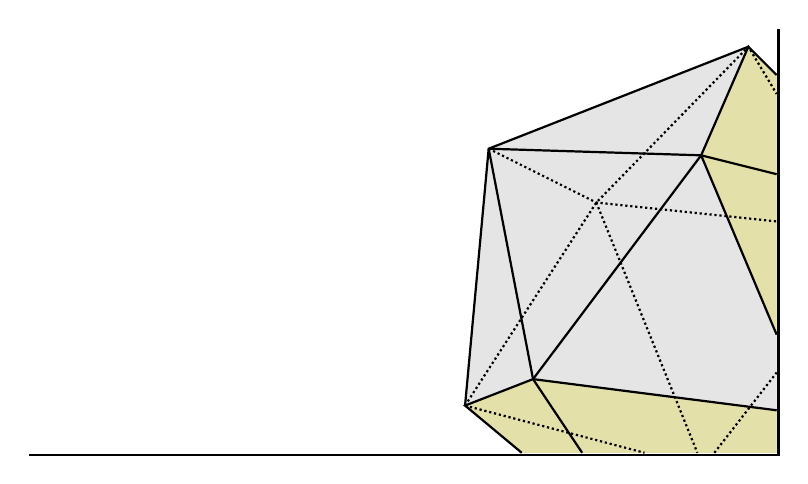
\begin{tikzpicture}[x=.012cm,y=.012cm,line width=.8pt]
\fill[gray!20] (470,75)--(495,347)--(770,455)--(800,425)--(800,25)--(530,25)--cycle;
\fill[olive!25] (720,340)--(770,455)--(800,425)--(800,25)--(530,25)--(470,75)--(542,103)--(800,70)--(800,150)--cycle;
\draw (8,23)--(802,23)--(802,474);
\draw (470,75)--(495,347)--(770,455)--(800,425);
\draw (495,347)--(720,340)--(800,320);
\draw (770,455)--(720,340)--(542,103)--(470,75)--(530,25);
\draw (495,347)--(542,103)--(594,25);
\draw (542,103)--(800,70);
\draw (720,340)--(800,150);
\draw[densely dotted] (495,347)--(609,290)--(800,270);
\draw[densely dotted] (470,75)--(609,290)--(770,455)--(800,405);
\draw[densely dotted] (609,290)--(716,25);
\draw[densely dotted] (470,75)--(660,25);
\draw[densely dotted] (734,25)--(800,110);
\end{tikzpicture}}

\scanpage{2}
\mspage{1}
\textcircled{1} Soit $\overline{\mathbf Q}$ la clôture algébrique de $\mathbf Q$ dans $\mathbf C$.
Si $\unsure{X=}\overline X$ est un schéma sur $\overline{\mathbf Q}$, on considère le
groupe $\mathcal G_{\overline X}$ des automorphismes de $\overline X$ en tant
que schéma absolu. On a une suite
\[
(1)\qquad 1\longrightarrow G_{\overline X}\longrightarrow\mathcal G_{\overline X}\longrightarrow\Gamma
\]
\margin{Question : \unsure{comme} \illegible{1} ?}
où
\[
(2)\qquad\left\{\begin{aligned}
\Gamma&=\operatorname{Gal}(\overline{\mathbf Q}/\mathbf Q),\\
G_{\overline X}&=\operatorname{Aut}(\overline X/\overline{\mathbf Q})
\end{aligned}\right.
\]
\margin{\diagram{\begin{tikzcd}[ampersand replacement=\&]
\overline{\mathbf Q}\arrow[r,hook]\arrow[d,phantom,"\cup" description]\&\Gamma(\unsure{X},\mathcal O_{\unsure{X}})\\
\mathbf Q\&
\end{tikzcd}}
\unsure{Il faut supposer} p.ex. que $\overline{\mathbf Q}$ est la
\unsure{clôt. int.} de $\mathbf Q$ ds $\unsure{\Gamma_X}$.}
Les sous-extensions $K$ de $\overline{\mathbf Q}/\mathbf Q$ correspondent
aux sous-groupes fermés $\Gamma_K$ de $\Gamma$ (d'indice
fini ssi $K$ fini sur $\mathbf Q$). À une restriction
du corps de base $\overline{\mathbf Q}$ de $\overline X$ à $K$ correspond
un relèvement
\[
(\unsure{4})\qquad
\diagram{\begin{tikzcd}[ampersand replacement=\&]
\mathcal G_{\overline X}\arrow[r,dash]\&\Gamma\arrow[d,phantom,"\cup" description]\\
\&\Gamma_K\arrow[ul]
\end{tikzcd}},
\]
\margin{\unsure{grain de sel d'effectivité de descente} \unsure{de gr. prof.}}
qui le définit si $\overline X$ est réduit\margin{?} et loc. de t.f.
sur $\overline{\mathbf Q}$. Cela montre que si $\overline X$ est de t.f.
\deleted{\unsure{quasi-proj.}}
sur $\overline{\mathbf Q}$, l'hom $\mathcal G_{\overline X}\mathbin{\unsure{-|\to}}\Gamma$ a une image
d'indice fini (puisqu'on peut \inserted{alors} réduire le
corps de base à une ext. finie $K$ de $\mathbf Q$).

\textcircled{2} \uline{Supposons $X$ connexe} \deleted{\unsure{et}}\inserted{$\ne\varnothing$}.
Considérons un revêtement universel $\widetilde X\xrightarrow{h}X$
\deleted{$X$}, et \deleted{considérons} posons
\[
(5)\qquad \mathcal E(X,\widetilde X)\ \unsure{\text{ou}}\ \mathcal E_X=\operatorname{Aut}(\widetilde X/X)
\]
\mspage{1}

\scanpage{3}
On a donc une suite exacte
\[
(6)\qquad\diagram{\begin{tikzcd}[ampersand replacement=\&]
1\arrow[r]\&\pi_1(X)\arrow[r]\arrow[d,equal]\&\mathcal E_X\arrow[r]\&\mathcal G_X\arrow[r]\arrow[d]\&1\\
\&\operatorname{Aut}(\widetilde X/X)\&\&\Gamma\&
\end{tikzcd}}
\]
\deleted{La donnée d'un point}

Considérons un point $\xi$
\[
(7)\qquad\xi\in X(\overline{\mathbf Q})
\]
et soit $\mathcal G_X(\xi)\subset\mathcal G_X$ le sous-groupe
de $\mathcal G_X$ qui fixe $\xi$. (NB. Si $G_X$ est
\margin{$X$ est de t.f. $/\overline{\mathbf Q}$ et \unsure{sép.}}
fini, $\mathcal G_X$ est profini et $\mathcal G_X(\xi)$ est un
s-groupe ouvert\unsure{\ldots}). On trouve alors,
si on choisit pour $\widetilde X$ le rev. universel
\inserted{$\widetilde X(\xi)$} pointé au dessus de $\xi$, un
splitting partiel de (6)
\[
(8)\qquad\diagram{\begin{tikzcd}[ampersand replacement=\&]
\mathcal E_X\arrow[r]\&\mathcal G_X\arrow[r,dash]\arrow[d,phantom,"\cup" description]\&1\\
\&\mathcal G_X(\xi)\arrow[ul]\&
\end{tikzcd}}
\]
Dans le cas où $\widetilde X$ est quelconque, on
ne trouve qu'un hom. mod conjugaison
\unsure{aux} autom intérieurs provenant de
$\pi_1(X)$. \deleted{Si $X$ est de t.f. et}
\mspage{2}

\scanpage{4}
\mspage{2}
\deleted{\unsure{s'immerge injectivement} dans un groupe algébrique
commutatif de rang unipotent nul
(i.e. ext. d'une VA par un tore) alors
\uline{l'application}}
\deleted{\diagram{\begin{tikzcd}[ampersand replacement=\&]
X(\overline{\mathbf Q})\arrow[r]\&{}
\end{tikzcd}}}

\textcircled{3} Supposons $X$ de t.f. sur $\overline{\mathbf Q}$. Alors on a
un ``germe de relèvement'' de $\Gamma$
\[
(9)\qquad\diagram{\begin{tikzcd}[ampersand replacement=\&]
\mathcal G_{\overline X}\arrow[r]\&\Gamma\arrow[d,phantom,"\cup" description]\\
\&\Gamma'\arrow[ul]
\end{tikzcd}}
\]
sur ss-groupe ouvert (modulo la relation
de coïncidence sur un ss groupe
ouvert plus petit). Pour \inserted{$\xi\in X(\overline{\mathbf Q})$ donné, et pour}
$\Gamma'$ assez petit,
$\Gamma'\mathbin{-}\mathcal G_{\overline X}$ se factorise par $\mathcal G_{\overline X}(\xi)$, de
\margin{$X=\overline X$}
sorte qu'on a un \inserted{germe d'} hom composé
\[
\deleted{\Gamma'\longrightarrow\mathcal E_X}
\qquad\inserted{\Gamma'\longrightarrow\mathcal E_X}
\]
rendant commutatif
\[
(10)\qquad\diagram{\begin{tikzcd}[ampersand replacement=\&]
\mathcal E_X\arrow[r]\&\mathcal G_X\arrow[r]\&\Gamma\\
\&\&\Gamma'\arrow[u,hook]\arrow[ull,"{\unsure{\varphi_\xi^t|\varphi_\xi}}"']
\end{tikzcd}}
\]
-- du moins si $\widetilde X=\widetilde X(\xi)$ -- sinon un
hom défini mod composition par un \unsure{autom}
int. provenant de $\pi_1(X)$. \unsure{Soulignons}
\mspage{3}

\scanpage{5}
encore une fois que c'est le \uline{germe}
seulement des $\varphi_\xi$ qui est défini
(\unsure{avec variation à} ss groupe d'indice
fini). [Si $X$ s'immerge injectivement
dans une extension d'une VA par un
tore, alors $\xi$ est connu quand on
connaît ce germe
\[
(11)\qquad\varphi_\xi\in\underset{\substack{\Gamma'\subset\Gamma\\\text{ouvert}}}{\lim\limits_{\longrightarrow}}
\operatorname{Hom}(\Gamma',\mathcal E_{\deleted{\unsure{\overline X}}\inserted{X}})
/\operatorname{Int}(\pi_1(X),\mathcal E_X)
\]
[et même l'image de $\varphi_\xi$ dans un $H^1$ abélien
convenable\unsure{\ldots}] ]

\textcircled{4}
\[
(12)\qquad\text{Soit }\boxed{D=\sum_{i\in I}D_i}\quad\text{un diviseur \inserted{effectif} sur }X,
\]
($I$ l'ens de ses comp. \unsure{irré d|irred}) sans comp. mult.,
supposons que $X$ soit régulier \inserted{(i.e. lisse)} en les
pts gén. de chaque $D_i$. Soit \deleted{$\unsure{X|X'}$}
\[
(13)\qquad X'=X-\operatorname{supp}D
\]
et considérons le sous-groupe $\mathcal G_{X';X}$ de
$\mathcal G_X$ qui invarie $D$. On le notera \inserted{encore} (par
abus de notation) $\mathcal G_{X'}$, \inserted{ou plus précisément $\mathcal G_{X'}(I)$.} Alors on a
\mspage{4}

\scanpage{6}
\mspage{3}
\[
(14)\qquad1\mathbin{\unsure{-|\to}}\pi_1(X')\mathbin{\unsure{-|\to}}\mathcal E_{X'}\longrightarrow\mathcal G_{X'}\longrightarrow1.
\]
et on a encore un germe de relèvement
(\unsure{éventuellement} mod comp. par autom int.
provenant de $\pi_1(X')$)
\[
(15)\qquad\diagram{\begin{tikzcd}[ampersand replacement=\&]
\mathcal E_{X'}\arrow[r,dash]\&\mathcal G_{X'}\arrow[r]\&\Gamma\arrow[d,phantom,"\cup" description]\\
\&\&\Gamma'\arrow[ull,"\varphi_\xi"']
\end{tikzcd}}
\]
(si $\xi\in X'(\overline{\mathbf Q})$).

Notons qu'on a ici un hom
\[
(16)\qquad\mathcal G_{X'}\longrightarrow\mathfrak S_I
\]
La théorie de Kummer nous fournit,
pour $\forall\,i$, un hom extérieur
\[
(17)\qquad\mathbf T(\overline{\mathbf Q})\xrightarrow{\varphi_i}\pi_1(X')
\]
\[
=\varprojlim\mu_n(\overline{\mathbf Q})
\]
\margin{$\varphi_i\in\operatorname{Homext}(\mathbf T(\overline{\mathbf Q}),\pi_1(X'))$}
\margin{\deleted{\unsure{il faut supposer} $\chi=1$ \unsure{si l'on veut}
\unsure{interpréter ça par} \illegible{6} \unsure{purement arithmétique} \illegible{3}}}
Notons aussi un hom canonique
\[
(18)\qquad(\mathcal G_{X'}\mathbin{-})\Gamma\xrightarrow{\chi}\widehat{\mathbf Z}^{*}\xrightarrow{\sim}\operatorname{Aut}(\mathbf T(\overline{\mathbf Q}))
\]
faisant opérer $\mathcal G_{X'}$ via $\Gamma$ sur $\mathbf T(\overline{\mathbf Q})$.
Ceci dit, l'opération extérieure de $\mathcal G_{X'}$
sur $\pi_1(X')$ est compatible avec la famille
\mspage{5}

\scanpage{7}
des $(\varphi_i)$ (``structure Kummérienne'')
compte tenu des opérations \inserted{(16) et (18)} de $\mathcal G_{X'}$
sur $I$ et $\mathbf T(\overline{\mathbf Q})$. On peut donc
écrire
\[
(19)\qquad\mathcal G_{X'}\longrightarrow\operatorname{Autext}(\pi_1(X'),\mathbf T(\overline{\mathbf Q}),(\varphi_i)).
\]
\deleted{Supposons $\unsure{X}$}

Soit $\widehat{\widetilde X'}$ le normalisé de $\deleted{\unsure{\widetilde{\phantom X}}}X$ dans ``l'extension
\unsure{étale|totale}'' définie par $\widetilde X'$, donc on a un
morphisme profini
\[
\widehat{\widetilde X'}\longrightarrow X
\]
Soit $\widetilde X'(I)$ l'image inverse de l'ens des
pts \deleted{génériques} \inserted{minimaux} de $D=\sum D_i$. On a
donc
\[
(20)\qquad\widetilde X'(I)\mathbin{-}I
\]
et une opération de $\deleted{\unsure{\mathcal G_{X'}}}\mathcal E_{X'}$ sur
$\widetilde X'(I)$ (par transport de structure)
compatible avec les opérations sur $I$
et l'application (20). Pour $i\in I$ soit
\[
(21)\qquad\widetilde X'(i)\subset\widetilde X'(I)
\]
sa fibre dans $\widetilde X'(I)$, \inserted{(c'est un espace hom.
sous $\pi_1(X')$. On trouve alors}
\mspage{6}

\scanpage{8}
\mspage{4}
une application
\[
(22)\qquad\widetilde X'(i)\xrightarrow{\Phi_i}\operatorname{Hom}(\mathbf T(\overline{\mathbf Q}),\pi_1(X'))
\]
\margin{\unsure{ici il est supposé} $\dim X=1$ -- autrement il
faut \unsure{voir|revoir} la définition de $\widetilde X'(I)$\ldots\
\unsure{Autre façon de dire : il faut que} $\widetilde X'$ \unsure{soit considéré}
\unsure{pour donner des} \illegible{1} \unsure{henséliens ou locaux au} dessus d'un \unsure{pt de} $X'(I)$\ldots}
compatible avec les opérations de $\pi_1(X')$
de part et d'autre, et qui précise
la donnée de $\varphi_i$ (17). Mieux encore,
le système $(\Phi_i)_{i\in I}=\Phi$ :
\[
(23)\qquad\widetilde X'(I)\xrightarrow{\Phi}\operatorname{Hom}(\mathbf T(\overline{\mathbf Q}),\pi_1(X'))
\]
est compatible avec les $\mathcal E_{X'}\deleted{\unsure{\mathcal E}}$ de part et
d'autre, en se rappelant, pour l'opération
de $\mathcal E_{X'}$ sur le mb de droite, de tenir
compte aussi de l'opération de $\mathcal E_{X'}$
sur $\mathbf T(\overline{\mathbf Q})$ (via $\Gamma$).

\textcircled{5} Soit enfin, par dessus le marché, une
partie $J\subset X'(\overline{\mathbf Q})$. Soit $\widetilde X'(J)$ son
image inverse dans $\widetilde X'$. Soit $\mathcal G_{X'}(I,J)$
ou simplement $\mathcal G'$ le sous-groupe de $\mathcal G_{X'}(I)$
qui invarie $J$. \deleted{\unsure{On voit les structures}} \inserted{Donc $\mathcal G'$}
opère sur $J$, sur $\widetilde X'(J)$ et sur
\[
(24)\qquad\widetilde X'(J)\longrightarrow J
\]
\mspage{7}

\scanpage{9}
Enfin, on a une famille de scindages \inserted{partiels}
\[
(25)\qquad\Psi^{\deleted{\unsure{\mathrm{ext}}}}=(\Psi_j)_{j\in J}:\bigl(\widetilde X'(j)\longrightarrow\operatorname{Hom}(\mathcal G'_j,\mathcal E'_{\deleted{\unsure{X'}}})\bigr)
\]
(où cette fois $\mathcal E'$ désigne l'image inverse
de $\mathcal G'\subset\mathcal G_{X'}$ dans $\mathcal E_{X'}$, \inserted{et $\mathcal G'_j$ le stab. de $j$ dans $\mathcal G'$}), compatible
avec les opérations de $\mathcal E'$ de part et
d'autre, \deleted{\unsure{se prolongeant} dans une famille de
scindages mod op. de $\pi_1$}
\[
\deleted{(26)\qquad\Psi^{\mathrm{ext}}=(\Psi_j^{\mathrm{ext}})_{j\in J}:\bigl(\widetilde X'(J)\longrightarrow\operatorname{Hom}(\mathcal G'_j,\mathcal E')/\operatorname{Int}(\pi_1,\mathcal E')\bigr)}
\]
\deleted{également compatible avec op. de $\mathcal E'$.}

\textcircled{6} \uuline{Récapitulons.} On se donne : \deleted{$X$
schéma de t.f. sur $\overline{\mathbf Q}$, un divi\unsure{-}}
\[
\mathrm I\quad\left\{\begin{array}{l}
X\text{ de t.f. sur }\overline{\mathbf Q}\\
D=\sum_{i\in I}D_i\text{ diviseur effectif sur }X\text{ à comp.}\\
\qquad\text{simples, }X\text{ lisse en les pts minimaux}\\
\qquad\text{de }\operatorname{supp}D\\
J\subset X'(\overline{\mathbf Q}),\quad\text{où }X'=X-D
\end{array}\right.
\]
On pose\margin{\unsure{(}}
\[
\mathrm{II}\quad\left\{\begin{array}{l}
\mathcal G'=\text{gr des autom du schéma \inserted{absolu} }X\\
\qquad\text{qui invarie }D\text{ et }J\\
G'=\text{ss-groupe de }\mathcal G'\text{ formé des }\overline{\mathbf Q}\text{-autom.}\\
\mathbf T(\overline{\mathbf Q})=\varprojlim_n\mu_n(\overline{\mathbf Q})\\[1ex]
\Gamma=\operatorname{Gal}(\overline{\mathbf Q}/\mathbf Q)
\end{array}\right.
\]
\mspage{8}

\scanpage{10}
\mspage{5}
d'où
\[
(1)\qquad1\longrightarrow G'\longrightarrow\mathcal G'\mathbin{\unsure{-|\to}}\Gamma
\]
et un germe de relèvement
\[
(2)\qquad\diagram{\begin{tikzcd}[ampersand replacement=\&]
\mathcal G'\arrow[r,dash]\&\Gamma\arrow[d,phantom,"\cup" description,"{\text{ss-groupe ouvert}}"']\\
\&\Gamma'\arrow[ul]
\end{tikzcd}}
\]
\margin{pour mémoire : relation avec \unsure{restrictions} des corps de base\ldots}
\uline{Choisissons} (cf normalisations plus bas)
\textcircled{III} \uline{un rev. universel} $\widetilde X'$ de $X'$,
d'où
\deleted{posons}
\[
\pi_1(X')=\operatorname{Aut}(\widetilde X'/X')
\]
On trouve alors

(3) \deleted{(3)} structure d'extension
\[
1\longrightarrow\pi_1(X')\mathbin{\unsure{-|\to}}\mathcal E'\mathbin{-}\mathcal G'\mathbin{-}1
\]
\margin{pour mémoire : relation entre pts de $X'(\overline{\mathbf Q})$ et scindages partiels de l'extension (3)\ldots}
\[
(4)\qquad\mathcal E'\text{-ensembles}\quad\left\{\begin{array}{l}\widetilde X'(I)\\\widetilde X'(J)\end{array}\right.
\]
(5) Opérations de $\mathcal E'$ sur $I,J$ via $\mathcal G'$, et
$\mathcal E'$-applications
\[
\left\{\begin{array}{l}
\widetilde X'(I)\mathbin{-}I\\
\widetilde X'(J)\mathbin{-}J\simeq\widetilde X'(J)/\pi_1
\end{array}\right.
\]
\mspage{9}

\scanpage{11}
(6) application
\[
\Phi:\deleted{\unsure{\operatorname{Hom}}}\widetilde X'(I)\mathbin{-}\operatorname{Hom}(\mathbf T(\overline{\mathbf Q}),\pi_1(X'))
\]
\margin{si $\dim X=1$ sinon il faut revoir avec plus de soin la situation\ldots}
compatible avec op. de $\mathcal E'$, opérant sur
le mb de droite grâce à ses op.
sur $\mathbf T(\overline{\mathbf Q})$ via ($\mathcal G'$ vi. $\Gamma$) et sur $\pi_1(X')$
[via autom int. dans (3)]

(7) \inserted{Syst. d'} applications
\[
\Psi=(\Psi_j^{\deleted{\unsure{\mathrm{ext}}}})_{j\in J}:\bigl(\widetilde X'(j)\longrightarrow\operatorname{Splitt}(\mathcal E'_j/\mathcal G'_j)\bigr)_{j\in J}\deleted{/\operatorname{Int}(\pi_1,\mathcal E')}
\]
compatibles aux opérations de $\mathcal E'_{\deleted{\unsure{j}}}$
(opérant sur le mb de droite grâce
aux autom intérieurs
\[
({}^g u)(\sigma)=g\,u(g_{\mathcal G'}^{-1}\sigma g_{\mathcal G'})\,g^{-1}
\]
où $\sigma\in\mathcal G'_{\unsure{gj|j}}$, $u\in\operatorname{Splitt}(\mathcal E'_j/\mathcal G'_j)$, $g\in\mathcal E'$,
$g_{\mathcal G'}\in\mathcal G'$ l'image de $g$ dans $\mathcal G'$).
\[
\deleted{(8)\quad\unsure{\Psi}=(\unsure{\Psi_j}):\bigl(\widetilde X'(\unsure{j})\longrightarrow\operatorname{Splitt}(\mathcal E'_j/\mathcal G'_j)\bigr)_{j\in J}}
\]
\margin{\deleted{(où $\mathcal G'_j$ est le stabilisateur de $j$ dans $\mathcal G'$, $\mathcal E'_j$ son
image inv. dans $\mathcal E'$ -- (8) ``\unsure{relevant|précisant}'' (7),
\unsure{après} $\mathcal G'_j$ et \unsure{conjugaison par} \unsure{$\pi_1$} dans $\mathcal E'$\ldots)}}
(9) germe d'homomorphisme
\[
\diagram{\begin{tikzcd}[ampersand replacement=\&]
\mathcal E'\arrow[r]\&\mathcal G'\arrow[r]\&\Gamma\arrow[d,phantom,"\cup" description]\\
\&\&\Gamma'\arrow[ull]\&\text{ss-groupe ouvert}
\end{tikzcd}}
\]
\mspage{10}

\scanpage{12}
\mspage{\unsure{6}}
Programme du \deleted{paradigme \unsure{de la théorie des|arithmétique des}} \inserted{``\unsure{gruppentheoretisches}} Gleichnis'' (paradigme en termes de théorie des groupes) de l'\inserted{arithmétique :}\deleted{\unsure{arithm.} géométrie algébrique absolue (en car. 0).}

a) Donner une description ``groupo-théorétique'' complète de $\Gamma$.

b) Donner une description complète de tous les éléments de structure énumérés ci-dessus, dans des cas typiques importants pour $(X,D,J)$, dont nous indiquons quelques-uns plus bas.

\margin{On \unsure{tâchera} de prendre $X$ \unsure{propre autant} que possible (quitte à \unsure{compléter}\ldots)}

\uline{NB} Quand on a les éléments de structure envisagés pour $(X,D,J)$, on les a aussi automatiquement pour $\forall$ rev.\inserted{étale} fini de $X'\ldots$ Il faudrait expliciter ce point avec soin, et expliciter également dans les $\unsure{=|2}$ optiques les foncteurs ``bouchage de trous'' (en rajoutant \inserted{certains} des $D_i$ qu'on avait \unsure{enlevés|exclus}) ou ``forage des trous'' \inserted{si $\dim X=1$} (en enlevant certains des $\xi\in J$).
\mspage{11}

\scanpage{13}
\uline{ReNB} Soit $\Gamma'$ un ss-groupe ouvert de $\Gamma$, correspondant à une ss-extension finie $K/\mathbf Q$ de $\overline{\mathbf Q}$, et considérons une \unsure{rationalisation} de la situation $(X,D,J)$ à $K$, donnée donc par un scindage partiel (cf (2))
\diagram{\begin{tikzcd}[ampersand replacement=\&]
\Gamma' \arrow[r,dash] \& \mathcal G'
\end{tikzcd}}
d'où une extension
\[
(9)\qquad
\diagram{\begin{tikzcd}[ampersand replacement=\&]
1 \arrow[r,dash] \& \pi_1(X') \arrow[r,dash] \& \mathcal E'_{\Gamma'} \arrow[r,dash] \& \Gamma' \arrow[r,dash] \& 1
\end{tikzcd}}
\]
Le groupe $\Gamma'$ opère donc sur $(X,D,J)$, donc sur \inserted{$X'$, donc sur} la catégorie des rev.\inserted{étales} finis de $X'$, (\deleted{\unsure{cat. que}} \inserted{qu'on} peut identifier à la cat. $\operatorname{Ens.f.}(\pi_1(X'))$. Pour $\forall\,\unsure{\gamma|\sigma}\in\Gamma'$, soit $B_\gamma$ le $\pi_1(X')$-bitorseur image inverse de $\gamma$ dans $\mathcal E'_{\Gamma'}$, il \deleted{définit} \inserted{explicite} l'opération de $\gamma$ sur $\operatorname{Rev\acute et}(X')\simeq\operatorname{Ens}(\pi_1)$ comme
\[
(10)\qquad E\longmapsto B_\gamma\mathbin{\wedge}_{\pi_1}E
\]
Si $\deleted{\unsure{D'}}Y'$ et ${}^{\gamma}Y'$ se correspondent, on a des isom. can. \deleted{\unsure{cat.}} \inserted{(tautologiques)}
\[
(11)\quad\left\{\begin{aligned}
Y'(I)&\simeq({}^{\gamma}Y')(I)\\
Y'(J)&=({}^{\gamma}Y')(J).
\end{aligned}\right.
\]
\mspage{12}

\scanpage{14}
\mspage{7}
En fait, si $Y'\longleftrightarrow E$, on a
\[
\begin{aligned}
Y'(I)&\simeq\widetilde X'(I)\mathbin{\wedge}_{\pi_1}E\\
Y'(J)&\simeq\widetilde X'(J)\mathbin{\wedge}_{\pi_1}E
\end{aligned}
\]
et \unsure{les} isomorphismes (11) reviennent à des iso.
\[
\left\{\begin{aligned}
\widetilde X'(I)\mathbin{\wedge}_{\pi_1}E&\simeq(\widetilde X'(I)\mathbin{\wedge}_{\pi_1}B_\gamma)\mathbin{\wedge}_{\pi_1}E\\
\widetilde X'(J)\mathbin{\wedge}_{\pi_1}E&\simeq(\widetilde X'(J)\mathbin{\wedge}_{\pi_1}(B_\gamma))\mathbin{\wedge}_{\pi_1}E
\end{aligned}\right.
\]
qu'on peut décrire à l'aide d'isom. de $\pi_1$-ens à droite
\[
\left\{\begin{aligned}
\widetilde X'(I)&\simeq\widetilde X'(I)\mathbin{\wedge}_{\pi_1}B_\gamma\\
\widetilde X'(J)&\simeq\widetilde X'(J)\mathbin{\wedge}_{\pi_1}B_\gamma
\end{aligned}\right.
\]
lesquels reviennent à la donnée d'hom.
\[
\left\{\begin{gathered}
\diagram{\begin{tikzcd}[ampersand replacement=\&]
B_\gamma \arrow[r,dash] \& \operatorname{Aut}_{\deleted{\unsure{\mathrm{ens}}}}(\widetilde X'(I))=\operatorname{Bij}(\widetilde X'(I),\widetilde X'(I))
\end{tikzcd}}\\
\text{et \unsure{itou|idem} pour }\widetilde X'(J)
\end{gathered}\right.
\]
compatibles avec les op de $\pi_1$ à g. et à dr.
Or la donnée de ces applications, pour $\gamma\in\Gamma'$ variable, équivaut \deleted{\unsure{peut se}} à la donnée d'\deleted{une}applications
\diagram{\begin{tikzcd}[ampersand replacement=\&]
\mathcal E'_{\Gamma'}=\displaystyle\bigcup_{\gamma\in\Gamma'}B_\gamma \arrow[r] \& \operatorname{Aut}_{\mathrm{ens}}(\widetilde X'(I))\\
{} \arrow[r] \& \operatorname{Aut}_{\mathrm{ens}}(\widetilde X'(J))
\end{tikzcd}}
et \unsure{celle qu'on cherche est} justement l'opération \unsure{déduite} par celles déjà \unsure{envisagées} de $\mathcal E'$ sur $\widetilde X'(I)$, $\widetilde X'(J)\ldots.$
\mspage{13}

\scanpage{15}
\textcircled{7} Réconstruction du \unsure{I|1}-groupoïde fondamental $\Pi_1(X';J)$ de $X'$, et des opérations de $\mathcal G'$ dessus, en termes de l'extension $\mathcal E'$ de $\mathcal G'$ par $\pi_1$, et de l'opération de $\mathcal E'$ sur $\widetilde X'(J)$ et $\widetilde X'(J)\longrightarrow J$ [et des applications (7) (8)
\diagram{\begin{tikzcd}[ampersand replacement=\&]
\Psi^{\unsure{\mathrm{ex}|\mathrm{ext}}}:\widetilde X'(J) \arrow[r] \& \operatorname{Splitt}(\mathcal E'/\mathcal G')/\pi_1
\end{tikzcd}}
\[
\Psi:\bigl(\diagram{\begin{tikzcd}[ampersand replacement=\&]
\widetilde X'(j) \arrow[r,dash] \& \operatorname{Splitt}(\mathcal E'_j/\mathcal G'_j)
\end{tikzcd}}\bigr)].
\]
\margin{inutile de se les donner, elles résultent des autres}
\[
\operatorname{Ob}\Pi_1=J
\]
\deleted{\unsure{Soit} $j,j'\in J$}

\uline{NB} si $\widetilde{\unsure{\xi|j}}\in\widetilde X'(J)$, $\widetilde X'[\unsure{j|\xi}]$ (rev universel de $X'$ en $\unsure{\xi|j}$) s'identifie à $\widetilde X'$ (puisque $\widetilde{\unsure{\xi|j}}$ est un pt marqué de $\widetilde X'$ au dessus de $\unsure{\xi|j}$
\diagram{\begin{tikzcd}[ampersand replacement=\&]
\widetilde X' \arrow[r,dash,"\unsure{\varphi|\Psi}_{\widetilde\xi}"] \& \widetilde X'[\unsure{j|\xi}]
\end{tikzcd}}
Si $\gamma\in\pi_1$, on aura
\[
\Psi_{\gamma\cdot\widetilde{\unsure{\xi|j}}}=\Psi_{\widetilde{\unsure{\xi|j}}}\circ\gamma_{\widetilde X'}^{\deleted{\unsure{-1}}}
\]
donc on peut écrire, indépendamment du choix du pt base $\widetilde{\unsure{\xi|j}}$
\diagram{\begin{tikzcd}[ampersand replacement=\&]
\widetilde X'[j] \& \underset{\text{torseur à dr sous }\pi_1}{\underbrace{\widetilde X'(j)}}\mathbin{\wedge}_{\pi_1}\widetilde X' \arrow[l,"\sim"']
\end{tikzcd}}
\mspage{14}

\scanpage{16}
\mspage{8}
Ceci noté, on aura donc, si $j,j'\in J=\operatorname{Ob}\Pi_1$
\[
\begin{aligned}
\operatorname{Isom}_{\Pi_{1,\unsure{\mathrm{é}|\phi}}}(j,j')&\overset{\mathrm{dfn}}=\operatorname{Isom}(\widetilde X'[j],\widetilde X'[j'])\\
&\simeq\operatorname{Isom}_{\pi_1\text{-tors à droite}}(\widetilde X'(j),\widetilde X'(j'))
\end{aligned}
\]
la composition des chemins étant la composition des hom de $\pi_1$-tors à droite.
\deleted{\unsure{Comme}} On a donc reconstruit \inserted{le groupoïde} $\Pi_1$ à l'aide de $\widetilde X'(J)$ et de l'opération libre (à droite) de $\pi_1$ sur $\widetilde X'(J)$.
\deleted{les opérations} Comment reconstituer l'opération de $\mathcal G'$ sur $\Pi_1$ ? L'opération sur $\operatorname{Ob}\Pi_1=J$ n'est autre que l'opération donnée de $\mathcal G'$ sur $J$ (factorisant celle de $\mathcal E'$). Soit $g\in\mathcal G'$, explicitons
\diagram{\begin{tikzcd}[ampersand replacement=\&]
\operatorname{Isom}_{\Pi_1}(j,j') \arrow[r,"g_{\Pi_1}","\sim"'] \arrow[d,equal] \& \operatorname{Isom}(gj,gj') \arrow[d,equal]\\
\operatorname{Isom}_{\pi_1}(\widetilde X'(j),\widetilde X'(j')) \arrow[r,"?","\sim"'] \& \operatorname{Isom}_{\pi_1}(\widetilde X'(gj),\widetilde X'(gj'))
\end{tikzcd}}
Pour ceci, considérons le \inserted{$\pi_1$-}bitorseur
\[
B_g\subset\mathcal E'\qquad\text{image inv. de }g\text{ par }\mathcal E'\mathbin{-}\mathcal G'
\]
On voit que l'on a (grâce à l'op. de $\mathcal E'$ sur $\widetilde X'(I)$]
\[
\begin{aligned}
\widetilde X'(gj)&\simeq\widetilde X'(j)\mathbin{\wedge}_{\pi_1}B_g\\
\widetilde X'(gj')&\simeq\widetilde X'(j')\mathbin{\wedge}_{\pi_1}B_g
\end{aligned}
\]
\mspage{15}

\scanpage{17}
d'où aussitôt la flèche envisagée.

Il faudrait encore expliciter comment (7) (8) résultent de la donnée de l'opération de $\mathcal E'$ sur $\widetilde X'(J)$, induisant une opération \uline{libre} de $\pi_1\subset\mathcal E'$ sur $\widetilde X'(J)$ (ayant $J$ comme ens quotient)\ldots.

\uline{Reformulation}

Considérons les systèmes
\[
\left\{\begin{gathered}
\diagram{\begin{tikzcd}[ampersand replacement=\&]
1 \arrow[r,dash] \& \pi \arrow[r,dash] \& \mathcal E \arrow[r,dash] \& \mathcal G \arrow[r,dash] \& 1 \& \text{ext. de groupes}
\end{tikzcd}}\\
Z\quad\mathcal E\text{-ens }\inserted{\ne\varnothing},\text{ où }\pi\subset\mathcal E\text{ opère librement}
\end{gathered}\right.
\]
Ils forment une \uline{catégorie} $C$.
Considérons les systèmes $(\Pi,\widetilde\Pi,p,\mathcal G,a)$ où $\Pi$ est un groupoïde \inserted{connexe}, $p:\widetilde\Pi\longrightarrow\Pi$ un rev. universel de $\Pi$, et $\mathcal G$ un groupe opérant \deleted{\unsure{sur}} sur $\Pi$ par automorphismes par $a:\mathcal G\longrightarrow\operatorname{Aut}(\Pi)$. Ils forment une catégorie $C'$. On va définir des équivalences quasi-inverses l'une de l'autre
\diagram{\begin{tikzcd}[ampersand replacement=\&]
C \arrow[r,shift left,"\alpha"] \& C' \arrow[l,shift left,"\beta"]
\end{tikzcd}}
\mspage{16}

\scanpage{18}
\mspage{9}
\uline{Définition de $\alpha$}\qquad On va définir
\[
\alpha(\mathcal E,\mathcal G,\pi,Z,\ldots)=(\Pi,\widetilde\Pi,p,\mathcal G,a)
\]
\[
\left\{\begin{array}{l}
\operatorname{Ob}\Pi=Z/\pi\quad(\text{soit }J)\\
\operatorname{Isom}(j,j')=\operatorname{Hom}_{\pi}(Z_j,Z_{j'})\\
\text{composition des flèches évidente}
\end{array}\right.\qquad\bigg|\quad\text{d'où groupoïde }\Pi
\]
\[
\deleted{\widetilde\Pi_j=Z_j}\qquad\operatorname{Ob}\widetilde\Pi=Z
\]
\diagram{\begin{tikzcd}[ampersand replacement=\&]
\operatorname{Isom}(z,z')=\{\unsure{k|*}\}\arrow[d]\&\begin{gathered}\forall z,z'\in Z\\(\widetilde\Pi\text{ cat. discrète})\end{gathered}\\
\operatorname{Isom}(j,j')\simeq\operatorname{Hom}(Z_j,Z_{j'})\&
\end{tikzcd}}
\deleted{(\unsure{où} $j,j'$ \unsure{les} \illegible{1})}\inserted{(où $j=\dot z$, $j'=\dot z'$)}
\margin{$\Longleftarrow$ $\widetilde\Pi$ cat. \uline{discrète} sur $\Pi$ définie par foncteur \inserted{contr.}
\diagram{\begin{tikzcd}[ampersand replacement=\&]
F:\Pi^\circ \arrow[r] \& \operatorname{Ens}
\end{tikzcd}}
$F(j)=Z_j,\ldots$\quad $\widetilde\Pi\simeq\Pi/F$}
$\downarrow$ transforme l'unique pt de $\operatorname{Hom}(z,z')$ en l'unique \inserted{$\pi$-}iso $Z_j\mathbin{-}Z_{j'}$ transformant $z$ en $z'\ldots.$

Pour l'instant on n'a pas utilisé $\mathcal E$ et l'op. de $\mathcal E$ sur $Z$. On va l'utiliser maintenant pour faire opérer $\mathcal G=\mathcal E/\pi$ sur $\Pi$, et $\mathcal E$ sur $\widetilde\Pi$, de façon compatible.
Comme $\mathcal E$ opère sur $Z=\operatorname{Ens}(\widetilde\Pi)$, il opère \unsure{en fait} sur $\widetilde\Pi$, cat. discrète associée, \deleted{\unsure{opérant librement}} et \deleted{le} $\pi$ opère par $\Pi$-auto---, d'où l'opération de $\mathcal G$ sur $\unsure{K|\Pi}$ par passage au quotient.
\mspage{17}

\scanpage{19}
\uline{Définition de $\beta$}\qquad On définit
\[
\beta(\Pi,\widetilde\Pi,p,\mathcal G,a)=(\mathcal E,\mathcal G,\pi,Z)\quad\text{ainsi :}
\]
$\mathcal E=$ groupe des couples $(g,\bar g)$, où $g\in\mathcal G$, $\bar g\in\operatorname{Aut}(\widetilde\Pi)$ compatible avec $g$
\[
\pi=\operatorname{Aut}(\widetilde\Pi/\Pi)
\]
$\mathcal E\mathbin{\unsure{-|\longrightarrow}}\mathcal G$ par $(g,\bar g)\longmapsto g$, d'où
\diagram{\begin{tikzcd}[ampersand replacement=\&]
1 \arrow[r,dash] \& \pi \arrow[r] \& \mathcal E \arrow[r,dash] \& \mathcal G \arrow[r] \& 1
\end{tikzcd}}
$Z=\operatorname{Ob}\widetilde\Pi$, avec opération évidente de $\mathcal E$ sur $Z\ldots$

Variantes profinies\ldots

\textcircled{8} Considérons, avec notations \unsure{du} \S 7,
\[
\left(\diagram{\begin{tikzcd}[ampersand replacement=\&]
1 \arrow[r,dash] \& \pi \arrow[r,dash] \& \mathcal E \arrow[r] \& \mathcal G \arrow[r,dash] \& 1
\end{tikzcd}}
\quad\text{et }Z\quad\mathcal E\text{-ens}\ne\varnothing\text{ sur lequel }\pi\text{ opère librement}\right)
\]
$\longleftrightarrow(\Pi,\widetilde\Pi,p,\mathcal G,a)$. On va interpréter la donnée d'un triple $(\inserted{\chi,}\tau,T,\Phi)$, où $\tau$ est un $\mathcal E$-ens, $T$ un groupe $(\simeq\widehat{\mathbf Z}\;?)$, \inserted{$\chi:\mathcal G\longrightarrow\operatorname{Aut}(T)$ \unsure{$(\simeq\widehat{\mathbf Z}^{*}\;\text{canon.}?)$}} et
\diagram{\begin{tikzcd}[ampersand replacement=\&]
\Phi:\tau \arrow[r] \& \operatorname{Hom}_{\mathrm{gr}}(T,\pi)
\end{tikzcd}}
compatible avec op. de $\mathcal E$ (opérant
\mspage{18}

\scanpage{20}
\mspage{10}
sur $\tau$ par l'op. donnée, et sur $\operatorname{Hom}_{\mathrm{gr}}(T,\pi)$ en considérant $T$, $\pi$ comme des $\mathcal E$-groupes grâce à $\chi$ et à l'opération de $\mathcal E$ sur $\pi$ par autom intérieurs\ldots Pour
\deleted{\deleted{ceci on introduit}
\[
J=\tau/\pi
\]
sur lequel $\mathcal E/\pi$ \inserted{qui est $\mathcal G$} opère par passage au quotient, $\tau\longrightarrow J$ devenant donc un $\mathcal E$-morphisme. Considérons alors le groupoïde $\langle T,J\rangle$ défini par
\[
\operatorname{Ob}\langle T,J\rangle=J
\]
\[
\operatorname{Isom}(j,j')=\left\{\begin{array}{ll}
\varnothing&\text{si }j\ne j'\\
T&\text{si }j=j'
\end{array}\right.
\]
composition des flèches étant celle de $T$. On a une opération de $\mathcal G$ sur $\langle T,J\rangle$ via ses opérations sur $T$ \inserted{(par $\chi$)} et sur $J$. On va définir un $\mathcal G$-morphisme de groupoïdes
\diagram{\begin{tikzcd}[ampersand replacement=\&]
\langle T,J\rangle \arrow[r] \& \Pi^\wedge
\end{tikzcd}}
où $\Pi^\wedge$ est le groupoïde des rev. \inserted{\unsure{0-conn.}} universels de $\Pi$, identifiable (via $\widetilde\Pi$ qui est un \unsure{$\in\Pi^\wedge$}) au groupoïde des}
\mspage{19}

\scanpage{21}
\deleted{$\pi$-torseurs. Pour $j\in J$, le $\pi$-torseur correspondant $P_j$ s'envoie dans $\tau_j=$ fibre de $j\in\tau_\pi$ dans $\tau$ \unsure{puis} la fibre de $P_j$ en $t\in\tau_j$ étant le torseur sur le stabilisateur $\pi_t$ de $t$ dans $\pi$ suivant :
on considère
\diagram{\begin{tikzcd}[ampersand replacement=\&]
\Phi(t):T \arrow[r] \& \pi
\end{tikzcd}}
alors $\pi_t$ centralise}

Considérons la restriction de l'opération de $\mathcal E$ sur $\tau$ à $\pi$, d'où un groupoïde $\langle\tau,\pi\rangle$ dont l'ens des objets est $\tau$, l'ens des $\operatorname{Isom}(t,t')$ étant
\[
\pi_{t\to t'}=\{\lambda\in\pi\mid\lambda t=t'\}.
\]
\deleted{\unsure{Les composantes}} On a
\[
\pi_0\langle\tau,\pi\rangle=\tau/\pi\overset{\mathrm{dfn}}=J
\]
\[
\pi_1(\tau,t)=\pi_t\quad(\text{stabilisateur de }t\text{ dans }\pi)
\]
et on trouve que $\pi_t$ centralise $\Phi(t)(T)\subset\pi$. On suppose \uline{$T$ commutatif} et $\deleted{\pi_t=\Phi_t(T)}\quad\Phi_t:T\xrightarrow{\sim}\pi_t$ --- \unsure{en d'autres termes on suppose donné}, en plus de $\tau$ $\mathcal E$-ens \unsure{donc|de} $\pi$-ens,
\mspage{20}

\scanpage{22}
\mspage{11}
un syst. transitif d'iso entre les $\pi_t$ $(t\in\tau)$, permettant de les identifier tous à un $=T$. Ainsi $\langle\tau,\pi\rangle$ devient un $T$-groupoïde, \unsure{i.e.|c.àd.} un groupoïde (pas néc. connexe) où les grpes fondamentaux des comp. conn. sont comm. et tous identifiés à $T$.
De plus, $\mathcal E$ opère sur ce $T$-groupoïde (en opérant également sur $T$) via ses opérations sur le système $(\tau,\pi)$ ($\pi$-\unsure{espace|ens} à gauche) en opérant sur $\tau$ par l'op. donnée et sur $\pi$ via autom int. de $\mathcal E$, enfin sur $T$ via $\mathcal G$ via $\chi\ldots.$

[Si $\mathcal E$ opère sur $\tau$, \unsure{restreignant} cette op. à $\pi$ on trouve un groupoïde $\langle\tau,\pi\rangle$ sur lequel $\mathcal E$ opère. Supposant ce groupoïde abélien, on a donc une famille de groupes abéliens \inserted{$(T_j)_{j\in J}$} indexée par $J=\tau/\pi$, sur laquelle opère $\mathcal E$ via $\mathcal E/\pi=\mathcal G$. Ceci dit, on suppose donné une trivialisation de cette famille $(T_j)$ par $T\simeq T_j$, compatible avec op. de
\mspage{21}

\scanpage{23}
$\mathcal G$ --- lequel opère donc sur $T$. Ceci donne naissance automatiquement à
\diagram{\begin{tikzcd}[ampersand replacement=\&]
\Phi:\tau \arrow[r,dash] \& \operatorname{Hom}_{\mathrm{gr}}(T,\pi)
\end{tikzcd}}
\ldots

Ceci dit, on a un hom du groupoïde $\langle\tau,\pi\rangle$ dans le groupoïde des rev. universels de $\Pi$, constant sur les objets et de valeur $\widetilde\Pi$ sur ceux-ci, qui envoie donc l'ens des flèches dans $\pi$ --- et qui pour $t,t'\in\tau$, désignant par $\pi_{t,t'}$ \inserted{$=\operatorname{Isom}_{\langle\tau,\pi\rangle}(t,t')$} l'ens des $\lambda\in\pi$ tels que $\lambda t=t'$, est l'inclusion de $\pi_{t,t'}$ dans $\pi$. Ce foncteur
\diagram{\begin{tikzcd}[ampersand replacement=\&]
\langle\tau,\pi\rangle \arrow[r] \& \begin{gathered}\text{Cat des rev. universels}\\\text{de }\Pi\text{ égaux à }\widetilde\Pi\\\simeq(\text{un objet et groupe d'isom--- }\pi)\end{gathered}
\end{tikzcd}}
est évidemment compatible avec op. de $\mathcal E$ sur $\unsure{\Pi|\widetilde\Pi}$ donc sur $\unsure{K|\pi}\ldots$
\mspage{22}

\scanpage{24}
\mspage{12}
Inversement, donnons-nous \inserted{un groupe $T$ abélien} un $T$-groupoïde \deleted{\unsure{connexe}} $\Lambda$, une opération de $\mathcal E$ sur $(T,\Lambda)$, et un hom de groupoïdes
\diagram{\begin{tikzcd}[ampersand replacement=\&]
\Lambda \arrow[r,"\text{foncteur \uuline{fidèle}}"] \& \begin{gathered}\text{groupoïde à un seul objet}\\\text{des rev. universels de}\\\Pi\text{ égaux à }\widetilde\Pi\\\text{dont les autom sont }\pi\end{gathered}
\end{tikzcd}}
compatible avec action de $\mathcal E$.
Soit $\tau=\operatorname{Ob}\Lambda$ [donc $\tau$ est un $\mathcal E$-ens], et pour $\forall\,t,t'\in\tau$, on a un hom \uline{injectif}
\diagram{\begin{tikzcd}[ampersand replacement=\&]
\underbrace{\operatorname{Isom}_\Lambda(t,t')}_{\pi_{t,t'}} \arrow[r,hook] \& \pi
\end{tikzcd}}
compatible avec composition des isom.

On a exprimé la donnée d'un foncteur fidèle d'un groupoïde $\Lambda$ dans $\langle\pi\rangle$ --- \deleted{Mais} [il faut se donner une famille de sous groupes $(\pi_t)_{t\in\tau}$ de $\pi$ et \unsure{d'ens vides ou} bitorseurs sous les $\pi_{t'},\pi_t\ldots$] On va maintenant introduire les op. de
\mspage{23}

\scanpage{25}
$\pi$ sur $\Lambda$, compatibles avec ses op. sur $\pi$ par autom int. Pour ceci, on va exiger
\[
\left\{\begin{gathered}
\forall t\in\tau=\operatorname{Ob}\Lambda,\quad\text{la famille des}\\
\pi_{t,t'}\subset\pi\quad(t'\in\tau\text{ variable})\text{ forme une}\\
\text{pseudo-partition de }\pi,\text{ i.e. }\forall\lambda\in\pi,\\
\exists\text{ un unique }t'\text{ tel que }\lambda\in\pi_{t,t'},\\
\text{i.e. une unique flèche de }\Lambda\text{ au-dessus}\\
\text{de }\lambda\text{ qui soit d'origine }t.
\end{gathered}\right.
\]
\margin{examinons à part \unsure{ce|cette} condition $\exists!$ de remontage des flèches à origine \unsure{remontée}, pour un morphisme de groupoïdes\ldots}
ce qui donne l'opération de $\pi$ sur $\unsure{\underset{t}{\tau}|\tau}=\operatorname{Ob}\Lambda$, et la façon de reconstituer
\[
\Lambda\simeq\langle\tau,\pi\rangle
\]
et le foncteur $\Lambda\longrightarrow\langle\pi\rangle$. \uline{On} \deleted{\illegible{1}} suppose de plus que les stabilisateurs $\pi_t$ sont abéliens, d'où une famille de groupes $(T_j)_{j\in J=\tau/\pi}$ et opérations de $\mathcal E$ sur $(T,\Lambda)$, de sorte que $\Lambda\longrightarrow\langle\pi\rangle$ soit compatible avec op. de $\mathcal E$\ldots

Ce n'est pas bien élucidant --- peut-être est-il plus agréable de
\mspage{24}

\scanpage{26}
\mspage{13}
considérer que \deleted{\unsure{le|que}} $\tau$ définit \inserted{(grâce à l'op. de $\pi$)} un foncteur
\diagram{\begin{tikzcd}[ampersand replacement=\&,row sep=large,column sep=huge]
\operatorname{Rev}(\Pi) \arrow[r,"F"] \& (\operatorname{Ens})\\
(\pi\text{-}\operatorname{Ens}) \arrow[u,"\simeq"',"\begin{gathered}\deleted{\text{via }\widetilde\Pi}\\E\longmapsto\widetilde\Pi^{\circ}\times_\pi E\end{gathered}"] \arrow[ur,bend right=25,"E\longmapsto\tau^{\circ}\wedge_\pi E"']
\end{tikzcd}}
[\uline{NB} l'indice $\circ$ indique qu'on a renversé les op. de $\pi$, pour faire opérer $\pi$ à dr)
foncteur commutant aux $\varinjlim$ quelconques. Ceci dit, on veut que $\unsure{\Gamma|F}$ (qui opère sur $\operatorname{Rev}(\Pi)$ via ses opérations sur $\Pi$) soit compatible avec le foncteur $F$, i.e. qu'on ait des isom
\[
F({}^{\gamma}\Pi')\simeq F(\Pi')
\]
$(\Pi'\in\operatorname{Ob}\operatorname{Rev}\Pi)$ fonctoriels en $\Pi'$, et avec transitivité pour $\gamma$ variable. On trouve que celà \unsure{s'exprime}
\mspage{25}

\scanpage{27}
que l'opération de $\pi$ sur $\tau$ a été prolongée en une opération de $\mathcal E$ sur $\tau$. Mais ceci ne donne pas d'interprétation \unsure{symp.} de la $T$-structure\ldots
\figure{\begin{tikzpicture}\draw (0,0)--(1.5,0);\end{tikzpicture}}

\textcircled{9} Les schémas et Topos fondamentaux dans la théorie.

\textcircled{A} \deleted{Topos \unsure{Etendus|Etendue}} \inserted{Topos} modulaires \inserted{$(\mathcal T_{0,\nu})_{\overline{\mathbf Q}}$} pour les courbes de genre $0$ avec $\nu$ points marqués, et famille \deleted{des} modulaire \deleted{\unsure{par}} $\nu$-ponctuée sur $M_{0\nu}$\ldots

Le Topos $(\mathcal T_{0,\nu})_{\mathbf Q}$ pour $\nu=0,1,2$ \uline{n'est} pas un étendu --- car le schéma d'Isom \unsure{d'un|d'une} $X/S$ fibré projectif de rang $1$, avec $\nu$ sections marquées (distinctes sur chaque fibre) est lisse de dim rel. $3-\nu\deleted{\unsure{\geq|=}}>0$ (si $\deleted{\unsure{\nu}}0\leq\nu\leq2$).
\deleted{Néanmoins} \inserted{En fait} ce sont les topos
\[
B_{\unsure{\operatorname{GP}(1)|\operatorname{PGL}(1)}},\quad B_{\operatorname{Aff}(1)},\quad B_{G_m},\quad\inserted{B_e=e}
\]
dont les
\mspage{26}

\scanpage{28}
\mspage{14}
groupes fondamentaux sont triviaux :
\margin{car \unsure{grps connexes}}
\[
\pi_1(\mathcal T_{0\nu})=0\qquad 0\leq\nu\leq3
\]
Le Topos $\mathcal T_{0,\nu}$ \deleted{est le topos fibré} \inserted{$(\nu\geq4)$ correspond au} \deleted{étale de} \inserted{schéma} des syst. de $\nu-3$ points distincts $(x_1,\ldots,x_{\nu-3})$ dans
\[
\mathbf P^1-\{0,1,\infty\}=E^1\setminus\{0,1\}.
\]
Son groupe fondamental est \inserted{le complété profini d'}un groupe de tresses $\Pi_{0,\nu}$, lequel (\unsure{en t.q.} que ``groupe extérieur'') dépend contra-fonctoriellement de $[1,\nu]$ pour les monomorphismes.

Sur $(\mathcal T_{0,\nu})_{\mathbf Q}$ on \inserted{\unsure{donc}} fait opérer \inserted{$(\mathcal T_{0,\nu})_{\overline{\mathbf Q}}$} $\mathfrak S_\nu$, donc $\mathfrak S_\nu\times\Gamma$ opère sur $\mathcal T_{0,\nu}$,
\figure{
\begin{tikzpicture}[x=1cm,y=1cm]
\fill (0,0) circle (.08);
\fill (.85,.15) circle (.085);
\fill (1.75,.3) ellipse (.21 and .24);
\fill (1.05,-.27) circle (.018);
\fill (1.42,-.34) circle (.035);
\end{tikzpicture}}
\mspage{27}

\scanpage{29}
\mspage{15}
\textcircled{9} \uline{Une conjecture arithmético-géométrique}

Soient $g,\nu\geq0$ des entiers. On désigne par $M_{g,\nu}$ le topos modulaire \inserted{sur $\mathbf Q$} pour les courbes \inserted{relatives} lisses propres relativement connexes de genre $g$, \uline{munies} de \deleted{\unsure{un}} $\nu$-uple de \unsure{$\nu$ sections|sections} disjointes sur chaque fibre. Sauf pour $g=0$, $\nu=0,1,2$ et $g=1$, $\nu=0$, ce topos est associé à une étendue algébrique, \unsure{notion proche = schémable}.

On a un hom naturel \deleted{\unsure{extér.}}
\[
\pi_1(M_{g,\nu};\xi)\longrightarrow\operatorname{Autextloc}^{\circ}\bigl(\pi_1(\overline X\setminus\{x_1,\ldots,x_\nu\})\bigr)\tag{1}
\]
où $(X;x_1,\ldots,x_\nu)$ est la courbe \inserted{(sur $\overline{\mathbf Q}$)} de genre $g$ avec $\nu$ pts marqués associée à $\xi$ \inserted{$\in M_{g,\nu}(\overline{\mathbf Q})$}. \deleted{\unsure{On}} L'exposant $\circ$ marque le fait qu'on prend les autom de $\pi_1$ qui n'échangent pas entre eux les classes de Cartan associés aux $x_i$.
\margin{il faut peut-être être plus \unsure{strict}, et exiger la commutation \unsure{:} des opérations \unsure{:} \unsure{définies} de $\mathfrak S_\nu$ sur le $\pi_1$ ?? Il faut regarder surtout le cas $g=0,\nu=3$\ldots}

Notons qu'on a aussi
\[
\pi_1(\overline M_{g,\nu};\unsure{\xi|j})\longrightarrow\operatorname{Autextloc}^{\circ\circ}\bigl(\pi_1(X\setminus\{x_1,\ldots,x_\nu\})\bigr)\tag{2}
\]
où le double $\circ$ indique qu'on prend des autom \inserted{\uline{stricts}} compatibles avec la structure \unsure{locale}, i.e. induisant l'identité sur $T=\operatorname{Tate}(\overline{\mathbf Q})$\ldots
\margin{Aut. \uline{\unsure{orientés}}}
\[
\pi_1(\unsure{M_{g,\nu}^{an}|\overline M_{g,\nu}};\unsure{\xi|j})\longrightarrow
\underbrace{\operatorname{Autextloc}^{\circ\circ}\Pi_1(\unsure{X^{an}|\overline X}\setminus\{x_1,\ldots,x_\nu\})}_{=\Gamma_{g,\nu}\ (\text{Teichmüller})}\tag{2 bis}
\]
dont on sait (théorie top.) que c'est un
\mspage{28}

\scanpage{30}
\uline{isomorphisme}, et dont (2) se déduit en passant au profini. On a ainsi un \inserted{hom de} suites exactes
\margin{sauf si $g=0,\nu=0,1,2$\quad\figure{\begin{tikzpicture}\node[draw,ellipse] {$g=1,\nu=0$};\end{tikzpicture}}?}
\diagram{\begin{tikzcd}[ampersand replacement=\&,column sep=small,row sep=large]
1 \arrow[r,dash] \& \pi_1(\overline M_{g,\nu};\unsure{\xi|j}) \arrow[r,dash] \arrow[d,"\simeq"',"\deleted{\unsure{\widehat\Gamma_{g\nu}}}"] \& \pi_1(M_{g,\nu};\xi) \arrow[r] \arrow[d] \& \Gamma \arrow[r,dash] \arrow[d,bend left=20] \& 1\\
1 \arrow[r] \& \widehat\Gamma_{g,\nu} \arrow[r] \& \operatorname{Autextloc}^{\circ}(\pi_1(X\setminus\{x_1,\ldots,x_\nu\})) \arrow[r] \& \operatorname{Aut}T \arrow[d]\\
\&\&\&1
\end{tikzcd}}\hfill(4)
\unsure{admettons} que $\widehat\Gamma_{g,\nu}$ est invariant dans $\operatorname{Autextloc}^{\circ}(\ ?\ )$.
\margin{Version corrigée éventuelle : $\pi_1(M_{g,\nu};\unsure{\xi|j})\simeq$ Normalisateur de $\widehat\Gamma_{g,\nu}$ dans $\operatorname{Autextloc}^{\circ}(\pi_1(X\setminus\{x_1,\ldots,x_\nu\}))$ induisant des \unsure{autom} de $\widehat\Gamma_{g,\nu}$ commutant à $\mathfrak S_\nu$ et préservant une structure ``locale'' éventuelle\ldots $*$}

On \deleted{\unsure{a}} aimerait que la flèche (1) (la flèche verticale centrale de (5)) soit un \uline{iso}. Cela donnerait une caractérisation de $\Gamma$ comme
\[
\operatorname{Autextloc}^{\circ}\left(\underbrace{\pi_1(\unsure{X^{an}|\overline X}\setminus\{x_1,\ldots,x_\nu\})^{\wedge}}_{\text{groupe standard}\ \text{bien connu}}\right)/\widehat\Gamma_{g,\nu}
\]
\margin{Pour $(g,\nu)$ sauf $g=0,\nu=0,1,2$\quad $g=1,\nu=0$ (cas où $\unsure{\pi_1(X_{\overline{\mathbf Q}}\setminus S_\nu)|\pi_1(X\setminus S_\nu)}$ \unsure{est un groupe abélien}). \deleted{\unsure{abélien} $*$ \unsure{est} \illegible{1}}}
\margin{Pour le cas $g=0,\nu=3$, il convient aussi d'être prudent et d'exiger des conditions de commutations avec op. ext. de $\mathfrak S_3$\ldots}

\uline{Ex} Pour $g=0,\nu=3$ celà donnerait l'expression déjà envisagée de $\Gamma$ comme
\[
\operatorname{Autextloc}^{\circ}\bigl(\pi_1(\mathbf P^1\setminus\{0,1,\infty\})\bigr).
\]
\mspage{29}

\scanpage{31}
\mspage{16}
Si on considère le quotient \inserted{$N_{g,\nu}$} de $M_{g,\nu}$ par $\mathfrak S_\nu$ (de sorte que $M_{g,\nu}$ est un rev. de groupe $\mathfrak S_\nu$ de $N_{g,\nu}$) on a
\diagram{\begin{tikzcd}[ampersand replacement=\&,column sep=small]
1 \arrow[r,dash] \& \pi_1(\overline M_{g,\nu}) \arrow[r] \& \begin{gathered}\pi_1(N_{g,\nu};\xi)\\=\pi_1(\overline N_{g,\nu},\Gamma;\unsure{\xi|j})\\\Vert\\\pi_1(M_{g,\nu},\mathfrak S_\nu;\xi)\\=\pi_1(\overline M_{g,\nu},\mathfrak S_\nu\times\Gamma)\end{gathered} \arrow[r] \& \mathfrak S_\nu\times\Gamma \arrow[r] \& 1
\end{tikzcd}}\hfill(5)
structure d'extension un peu plus riche que la première ligne de (4). La conjecture faite équivaut à la suivante :
\[
\pi_1(N_{g,\nu};\xi)\xrightarrow{\sim}\operatorname{Autextloc}\bigl(\pi_1(X_{\unsure{\xi|j}}\setminus\{x_1,\ldots,x_\nu\})\bigr)
\]
ou encore
\[
\Gamma\simeq\operatorname{Autextloc}\bigl(\pi_1(X_{\unsure{\xi|j}}\setminus\{x_1,\ldots,x_\nu\})\bigr)/\widetilde\Gamma_{g,\nu}^{\wedge}
\]
où
\[
\widetilde\Gamma_{g,\nu}\simeq\operatorname{Autextloc}^{+}\bigl(\pi_1(X_{\unsure{\xi|j}}^{an}\setminus\{x_1,\ldots,x_\nu\})\bigr).
\]

$*$ NB Il faudrait déterminer le groupe des automorphismes \inserted{$G_{g,\nu}$} du topos modulaire géom $\overline M_{g,\nu}$ \deleted{\unsure{est}} ($G_{g,\nu}=\inserted{\operatorname{Im}}\mathfrak S_\nu$ ? \unsure{\}} Sans doute $\mathfrak S_\nu$ opère fidèlement sauf $g=0,\nu\leq4$\ldots)

\uline{Question}
\[
\Gamma\longrightarrow\operatorname{Autext}\left(\underbrace{\widehat\Gamma_{g,\nu}}_{\pi_1(\overline M_{g,\nu})}\right)
\quad\left\{\begin{array}{l}\text{injectif ?}\\\text{bijectif}\end{array}\right.
\]
\margin{(Sans doute \unsure{il faut} \unsure{condition} \unsure{sur le} \illegible{2}}
\mspage{30}

\scanpage{32}
\uline{Question}\quad $\operatorname{Autext}(\Gamma_{g,\nu})=1$ ?
\mspage{31}

\scanpage{33}
\margin{\begin{tabular}{c}
IBM\\IBM\\IBM\\IBM\\IBM\\IBM\\IBM\\IBM\\IBM\\IBM\\IBM\\IBM\\IBM\\IBM\\IBM\\IBM\\IBM\\IBM\\IBM\\IBM\\IBM\\IBM\\IBM\\IBM\\IBM\\IBM\\IBM\\IBM\\IBM\\IBM\\IBM
\end{tabular}}
\diagram{\begin{tikzcd}[ampersand replacement=\&,column sep=small,row sep=small]
1 \arrow[dr,dash] \& 1 \arrow[dr,dash]\\
1 \arrow[r] \& \pi_1(\overline X_{\unsure{g|\xi}}\setminus S_\nu) \arrow[r] \arrow[dr] \& \pi_1(\overline X_{\unsure{j|\xi}}-S_\nu) \arrow[r,dash] \arrow[dr] \& 1 \arrow[dr]\\
\&1 \arrow[r,dash] \& \pi_1(\overline M_{g,\nu+1}) \arrow[r] \arrow[dr] \& \pi_1(M_{g,\nu+1}) \arrow[r,dash] \arrow[dr] \& \Gamma \arrow[r,dash] \arrow[dr] \&1\\
\&\&1 \arrow[r,dash] \& \pi_1(\overline M_{g,\nu}) \arrow[r,dash] \arrow[dr] \& \pi_1(M_{g,\nu}) \arrow[r] \arrow[dr,Rightarrow] \& \Gamma \arrow[r,dash] \arrow[dr,Rightarrow] \&1\\
\&\&\&\&1\&1\&1
\end{tikzcd}}
\diagram{\begin{tikzcd}[ampersand replacement=\&,column sep=small,row sep=small]
1 \arrow[dr,dash] \&1 \arrow[dr]\\
1 \arrow[r] \& \begin{gathered}\widehat\pi_{g,\nu}\\\deleted{\unsure{\pi_{g,\nu}}}\end{gathered} \arrow[r,"\sim"] \arrow[dr] \& \widehat\pi_{g,\nu} \arrow[r] \arrow[dr] \&1 \arrow[dr,dash]\\
\&1 \arrow[r,dash] \& \widehat\Gamma_{g,\nu+1} \arrow[r] \arrow[dr] \& \operatorname{Autloc}^{\circ}(\widehat\pi_{g,\nu})^{!} \arrow[r] \arrow[dr] \& \Gamma \arrow[r,dash] \arrow[dr,Rightarrow] \&1\&\Sigma_{\nu+1}\\
\&\&1 \arrow[r] \& \widehat\Gamma_{g,\nu} \arrow[r] \arrow[dr] \& \begin{gathered}\operatorname{Autextloc}^{\circ}(\widehat\pi_{g,\nu})^{!}\\\text{\unsure{traces|tresses}}\end{gathered} \arrow[r] \arrow[dr] \&\Gamma \arrow[r,dash] \&1\&\Sigma_\nu\\
\&\&\&\&1\&1
\end{tikzcd}}
\[
\begin{gathered}
M'_{g,\nu}(K)\ni\xi\\
\Gamma'_{g,\nu}\unsure{\ni|\supset}G_\xi
\end{gathered}
\]
\diagram{\ensuremath{\begin{array}{ccc}
\deleted{\unsure{\Gamma|\Sigma}}\ \widehat\Sigma_{g,\nu}^{\sim}&&\Sigma_{g,\nu}\\
\Vert&&\\
\overline\Sigma_{g,\nu}&&
\end{array}}}
\margin{\begin{tabular}{c}6\\5\\4\\3\\2\\1\\0\end{tabular}}
\margin{2975 -- 132}
\mspage{32}

\scanpage{34}
\diagram{\ensuremath{\begin{array}{rrrr}
************&0.0000&&\\
************&**********&&\\
************&**********&&\\
75.000&&&\\
0.0307&20.4842&0.9297&\\
0.0309&21.3976&0.9048&\\
0.0310&22.3325&0.8763&\\
0.0311&23.2828&0.8443&\\
0.0313&24.2418&0.8090&\\
0.0314&25.2032&0.7705&\\
0.0315&26.1611&0.7289&\\
0.0317&27.1095&0.6845&\\
0.0318&28.0431&0.6374&\\
0.0319&28.9568&0.5878&\\
0.0321&29.8459&0.5358&\\
0.0322&30.7065&0.4817&\\
0.0323&31.5349&0.4258&\\
0.0325&32.3279&0.3681&\\
0.0326&33.0829&0.3090&\\
0.0327&33.7976&0.2487&\\
0.0329&34.4703&0.1874&\\
0.0330&35.0994&0.1253&\\
0.0331&35.6839&0.0628&\\
0.0333&36.2229&0.0000&\\
0.0334&36.7160&-0.0627&\\
0.0335&37.1629&-0.1252&\\
0.0337&37.5634&-0.1873&\\
0.0338&37.9177&-0.2486&\\
0.0339&38.2260&-0.3089&\\
0.0341&38.4885&-0.3680&\\
0.0342&38.7058&-0.4257&\\
0.0343&38.8783&-0.4816&\\
0.0345&39.0067&-0.5357&\\
0.0346&39.0916&-0.5877&\\
0.0347&39.1337\smash{\raisebox{-.5\baselineskip}{$\inserted{\Big)\,\text{max}}$}}&-0.6373&\\
0.0349&39.1337&-0.6844&\\
0.0350&39.0925&-0.7289&\\
0.0351&39.0108&-0.7704&\\
0.0353&38.8894&-0.8089&\\
0.0354&38.7293&-0.8442&\\
0.0355&38.5313&-0.8762&\\
0.0357&38.2964&-0.9047&\\
0.0358&38.0256&-0.9297&\\
0.0359&37.7197&-0.9510&\\
0.0361&37.3799&-0.9685&\\
0.0362&37.0072&-0.9822&\\
0.0363&36.6027&-0.9920&\\
0.0365&36.1675&-0.9980&\\
0.0366&35.7027&-1.0000&\\
0.0367&35.2095&-0.9980&\\
0.0369&34.6893&-0.9921&\\
0.0370&34.1432&-0.9823&\\
0.0371&33.5725&-0.9686&\\
0.0373&32.9788&-0.9510&\\
0.0374&32.3633&-0.9298&\\
0.0375&31.7275&-0.9048&\\
0.0377&31.0730&-0.8763&\\
0.0378&30.4013&-0.8444&\\
0.0379&29.7141&-0.8091&\\
0.0381&29.0130&-0.7706&\\
0.0382&28.2999&-0.7290&\\
0.0383&27.5764&-0.6846&\\
0.0385&26.8445&-0.6375&\\
0.0386&26.1062&-0.5879&\\
0.0387&25.3634&-0.5359&\\
0.0389&24.6183&-0.4818&
\end{array}}}
\[
\begin{aligned}
\Delta U&=26.3878\ \unsure{\mathrm{m/s}|\mathrm{m/o}}\\
U_m&=\unsure{25.939|25.9398}\ \unsure{\mathrm{m/s}|\mathrm{m/o}}
\end{aligned}
\]
\diagram{\ensuremath{\begin{array}{r}
39.1337\\12.7459\\\hline26.3878
\end{array}}}
\diagram{\ensuremath{\begin{array}{r}
12.7459\\13.1939\\\hline25.9398
\end{array}}}
\mspage{33}

\cotefile{141}
\scanpage{1}
IMAG

INSTITUT MONTPELLIERAIN

ALEXANDER GROTHENDIECK

\figure{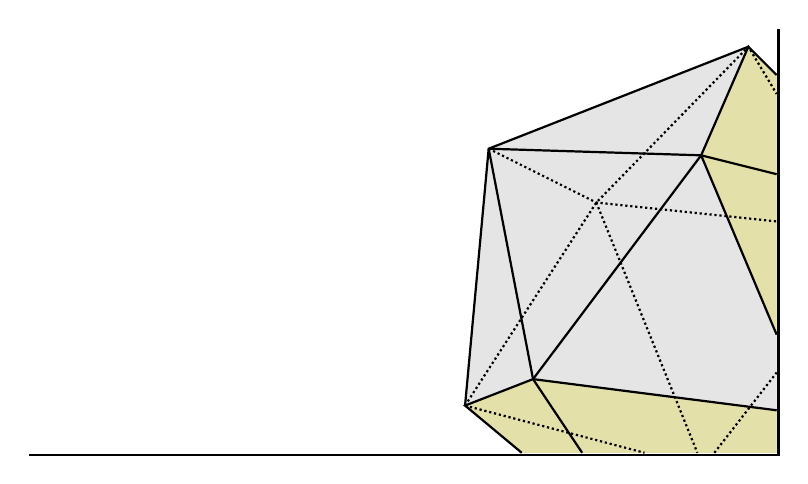
\begin{tikzpicture}[x=.012cm,y=.012cm,line width=.8pt]
\fill[gray!20] (470,75)--(495,347)--(770,455)--(800,425)--(800,25)--(530,25)--cycle;
\fill[olive!25] (720,340)--(770,455)--(800,425)--(800,25)--(530,25)--(470,75)--(542,103)--(800,70)--(800,150)--cycle;
\draw (8,23)--(802,23)--(802,474);
\draw (470,75)--(495,347)--(770,455)--(800,425);
\draw (495,347)--(720,340)--(800,320);
\draw (770,455)--(720,340)--(542,103)--(470,75)--(530,25);
\draw (495,347)--(542,103)--(594,25);
\draw (542,103)--(800,70);
\draw (720,340)--(800,150);
\draw[densely dotted] (495,347)--(609,290)--(800,270);
\draw[densely dotted] (470,75)--(609,290)--(770,455)--(800,405);
\draw[densely dotted] (609,290)--(716,25);
\draw[densely dotted] (470,75)--(660,25);
\draw[densely dotted] (734,25)--(800,110);
\end{tikzpicture}}

\scanpage{2}
$V$ : \uline{V.d. noethérien}, complet
\[
\operatorname{Spec}(V)\qquad k\ \text{\unsure{corps résid.}}\qquad K\ \text{\unsure{corps fractions}}
\]
\unsure{Groupe|Gpe} galoisien $(K)$

a) $\operatorname{car}(k)=0$\qquad \uuline{$k$ alg clos}
\figure{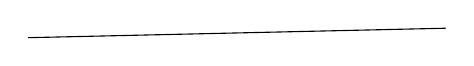
\begin{tikzpicture}\draw (0,0)--(5.3,.12);\end{tikzpicture}}
Les \unsure{extens|extensions} de $K$ sont \unsure{abél.} cycliques donc Kummeriennes.
\[
K^*/K^{*n}\simeq\mathbf Z/n\mathbf Z\qquad\text{(par la valuation)}
\]
Soit $\overline K$ clôture de $K$.
\diagram{\begin{tikzcd}[ampersand replacement=\&,column sep=small,row sep=small]
\Gamma(\overline K,K) \arrow[r,phantom,"\overset{\text{not}}{=}"] \& T_\infty(k) \arrow[r,phantom,"="] \& \displaystyle\varprojlim_n\underbrace{\mu_n(k)} \arrow[d,phantom,"\wr"] \& (\simeq\widehat{\mathbf Z})\\
\&\&\mathbf Z/n\mathbf Z
\end{tikzcd}}
\figure{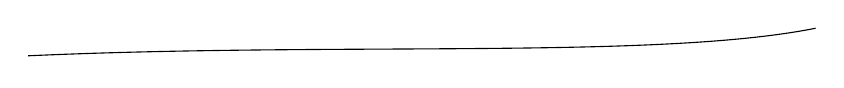
\begin{tikzpicture}\draw (0,0)..controls (4,.18) and (8,-.05)..(10,.35);\end{tikzpicture}}
Si $k$ car $\unsure{\ne0|p>0}$ $V$ pas \unsure{néces.} complet,
\[
\underset{\text{prem à }p}{\pi_1(K)}\longrightarrow\varprojlim_{n\text{ prem à }p}\mu_n(\unsure{k|K})
\]
\mspage{1}

\scanpage{3}
UNIVERSITE

DES SCIENCES ET TECHNIQUES

DU LANGUEDOC

\texttt{------------}

Service de la Scolarité

MA/GJ

Diffusion : Liste A

N° : 5982

Montpellier, le 12 Novembre 1980

AVIS DE SOUTENANCE D'UNE THESE DE DOCTEUR INGENIEUR

CHIMIE ORGANIQUE PHYSIQUE

\texttt{-------------------------}

\uline{Nom et prénom du candidat} : MAUBERT Claude

\uline{Titre de la thèse} : ETUDES CINETIQUES DES TELOMERISATIONS AMORCEES PAR LES SELS DE METAUX DE TRANSITION ET LES GENERATEURS DE RADICAUX LIBRES.

\uline{Date, lieu et heure de soutenance prévus} : 18 NOVEMBRE 1980 à 10 Heures 30 mn

E.N.S.C.M.

\uline{Nom du Directeur de thèse} : Monsieur le Professeur Y. PIETRASANTA

\uline{Désignation du laboratoire où la thèse est préparée} : Laboratoire de Chimie Appliquée

E.N.S.C.M. 8 Rue de l'Ecole Normale, 34075 MONTPELLIER CEDEX.

\uline{Résumé de la thèse} :

Cette thèse est axée sur la détermination des paramètres permettant de contrôler les réactions de télomérisation. Le cas des télomérisations par catalyse rédox des acrylates de méthyle et d'éthyle avec le tétrachlorure de carbone a d'abord été étudié. Il est apparu que les chlorures ferriques et cuivriques étaient les réactifs prépondérants pour le contrôle des degrés de polymérisation. On a ensuite mis en évidence une diminution de l'importance du transfert lorsque la longueur de la chaîne augmentait. Le dernier volet de cette étude concerne la télomé-\\
risation de l'acétate de vinyle avec le tétrachloro 2,4,4,4, butanoate de méthyle amorcée par l'azobisisobutyronitile. La constante de transfert au télogène a été calculée ; on a également évalué le pourcentage des chaînes macromoléculaires comportant une molécule de télogène en extrémité.

\uline{Durée approximative des recherches ayant abouti à la thèse} : 3 ans

\uline{Composition du jury proposé} :
\begin{tabular}{ll}
MM.&REMPP P.\\
& BOUTEVIN B.\\
& DEISS W.J.\\
& GENESTE P.\\
& PIETRASANTA Y.
\end{tabular}

P. le Secrétaire Général,

L'Attachée d'Administration Universitaire,

\uline{\unsure{P. Gentil|A. Gentil}}

\uline{A. GENTIL}
\mspage{2}

\scanpage{4}
\[
\bar s\in S\qquad
\pi_1(S,\bar s)\longrightarrow
\varprojlim_{n\ \unsure{\text{prem. à }S}}\mu_n(S)
\]
$\bar s$ \uline{pt géométr.}

\figure{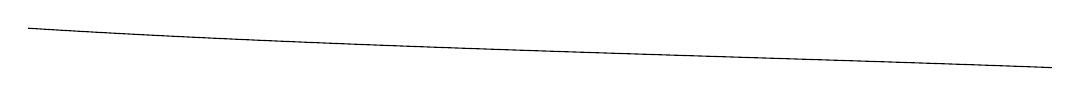
\begin{tikzpicture}
\draw (0,0.2) .. controls (4,-0.05) and (9,-0.15) .. (13,-0.3);
\end{tikzpicture}}

\diagram{\ensuremath{\begin{array}{ccccccccc}
1&\longrightarrow&\displaystyle\varprojlim_{n\ \unsure{\text{prem. à }p}}\mu_n(\bar k)&\unsure{\longmapsto}&\pi_1(K)&\longrightarrow&\pi_1(k)&\longrightarrow&1\\
&&&&&&\Vert&&\\
&&&&&&\pi_1(V)&&
\end{array}}}

\mspage{3}

\scanpage{5}
UNIVERSITE\\
DES SCIENCES ET TECHNIQUES\\
DU LANGUEDOC\\
\texttt{------------}\\
Service de la Scolarité\\
MA/GJ\\
Diffusion : Liste A\\
N\textdegree\ : 5890

Montpellier, le 7 Novembre 1980

AVIS DE SOUTENANCE D'UNE THESE DE DOCTORAT DE 3ème CYCLE

ECOLOGIE GENERALE ET APPLIQUEE Opt. ECOLOGIE TERRESTRE

\figure{\begin{tikzpicture}\draw (0,0)--(4,0);\end{tikzpicture}}

\uline{Nom et prénom du candidat} : MICHELLAND Dominique

\uline{Titre de la thèse} : SURVIE EN MILIEU INSULAIRE : QUELLE STRATEGIE ? LE CAS DES MESANGES EN CORSE.

\uline{Date, heure et lieu de soutenance prévus} :\\
17 NOVEMBRE 1980 à 15 Heures\\
Salle de cours n\textdegree\ 9 - USTL

\uline{Nom des Directeurs de thèse} :\\
MM. LEGENDRE et BLONDEL

\uline{Désignation du Laboratoire où la thèse est préparée} :\\
Laboratoire de Systématique et d'Ecologie Méditerranéennes

\uline{Résumé de la thèse} :

En Corse les populations de mésanges présentent un certain nombre de caractères démographiques et biométriques qui les différencient nettement des populations continentales.

A la lumière de la théorie de la biogéographie insulaire, cet ensemble d'observations peut s'interpréter comme le résultat de pressions de sélection de type K qui favorisent la survie des populations dans les milieux isolés et confinés.

Ce travail montre les répercussions, à l'échelle des populations, des importantes modifications, mises en évidence par ailleurs, de la structure et de la dynamique des communautés insulaires.

\uline{Durée approximative des recherches ayant abouti à la thèse} : 2 ans

\uline{Composition du jury proposé} :\\
MM. AMANIEU\\
\hspace*{2em}BLONDEL\\
\hspace*{2em}BOURLIERE\\
\hspace*{2em}THALER\\
\hspace*{2em}ISENMANN

P. le Secrétaire Général,\\
l' Attachée d'Administration Universitaire,

\uline{\unsure{P. Gentil|A. Gentil}}\\
\uline{A. GENTIL}

\figure{
\begin{tikzpicture}
\draw (0.3,2.5) arc[start angle=100,end angle=245,radius=1.55];
\draw[gray] (-0.97,1.8) .. controls (-1.2,1.2) and (-0.8,0.3) .. (-0.6,0);
\node[rotate=62] at (-0.95,1.95) {\unsure{ACAD}};
\node[rotate=-41] at (0.05,1.05) {\unsure{SCIENCES}};
\end{tikzpicture}}

\mspage{4}

\scanpage{6}
\diagram{\begin{tikzcd}[ampersand replacement=\&,column sep=small]
0\arrow[r]\&H^0(S,\mu_n)\arrow[r,dash]\&H^0(S,G_m)\arrow[r,dash]\&H^1(S,\mu_n)\arrow[r]\&H^1(S,G_m)
\end{tikzcd}}

\diagram{\begin{tikzcd}[ampersand replacement=\&,column sep=large]
\mu_{\unsure{n|1n}}(S)\arrow[r]\&G_m(S)\arrow[r]\&G_m(S)\arrow[r]\&\operatorname{Rev}(S,\mu_n)\arrow[d]\\
\&\&\&\operatorname{Pic}(S)\arrow[d]\\
\&\&\&\unsure{\operatorname{Pic}}^{\unsure{\otimes n}}(S)
\end{tikzcd}}

\diagram{\begin{tikzcd}[ampersand replacement=\&,column sep=large]
0\arrow[r,dash]\&G_m(S)_n\arrow[r]\&\operatorname{Rev}(S,\mu_n)\arrow[r]\&\unsure{{}_n\operatorname{Pic}}(S)\arrow[r]\&0
\end{tikzcd}}

\diagram{\begin{tikzcd}[ampersand replacement=\&,column sep=huge]
a\arrow[r,dash]\&\operatorname{Spec}\bigl(\underline{\mathcal O}_S[T]/T^n-a\bigr)
\end{tikzcd}}
\[
A[T]/(T^n-a)
\]

\mspage{5}

\scanpage{7}
UNIVERSITE\\
DES SCIENCES ET TECHNIQUES\\
DU LANGUEDOC\\
\texttt{------------}\\
Service de la Scolarité\\
MA/GJ\\
Diffusion : Liste A\\
N\textdegree\ : 5983

Montpellier, le 12 Novembre 1980

AVIS DE SOUTENANCE D'UNE THESE DE DOCTEUR INGENIEUR

SCIENCES ALIMENTAIRES Option GENIE ET TECHNOLOGIE ALIMENTAIRES -

FERMENTATIONS

\texttt{----------------------}

\uline{Nom et prénom du candidat} : COMTE Francis

\uline{Titre de la thèse} : Etude des isothermes d'adsorption de composés phénoliques.

\uline{Date, heure et lieu de soutenance prévus} : 18 NOVEMBRE 1980 à 15 Heures 30 mn\\
Salle de cours n\textdegree\ 9 - U.S.T.L.

\uline{Nom du Directeur de thèse} : Monsieur le Professeur J. CROUZET

\uline{Désignation du laboratoire où la thèse est préparée} : Biochimie Appliquée

\uline{Résumé de la thèse} :

Le tracé d'isothermes d'adsorption sur silice de composés phénoliques (acides benzoïque et salycilique) étudiés en qualité de modèles d'anthocyanes a été obtenu par des méthodes dynamiques mettant en oeuvre la chromatographie liquide haute performance.

Parmi les différentes méthodes utilisées par élution (profil de pic, maximum de pics) ou par analyse frontale (équilibre, profil de désorption) la technique du profil de désorption est la plus rapide mais sujette à cautions. La méthode la plus fiable, quoique la plus longue, est la méthode à l'équilibre, c'est d'ailleurs la seule méthode qui autorise le tracé des isothermes individuelles par adsorption d'un mélange.

Par modélisation nous avons pu montrer que le meilleur accord était obtenu avec le modèle de SCOTT et KUCERA qui décrivent une adsorption en double couche.
En dépit des difficultés qui se sont liées à l'intervention de phénomènes propres à la chromatographie liquide et qui contribuent à la déformation des pics il nous a été possible de montrer que la capacité d'adsorption de la silice était supérieure pour l'acide ben-\\
zoïque. Ceci est confirmé par l'étude de l'adsorption mixte sans que l'on puisse parler d'adsorption spécifique ou de sélectivité de l'absorbant.

\uline{Durée approximative des recherches ayant abouti à la thèse} : 3 ans

\uline{Composition du jury proposé} :\\
MM. ROUZAUD J.\\
\hspace*{2em}CROUZET J.\\
\hspace*{2em}GOMA G.\\
\hspace*{2em}COMBE P.

P. le Secrétaire Général,\\
L'Attachée d'Administration Universitaire,

\uline{\unsure{P. Gentil|A. Gentil}}\\
\uline{A. GENTIL}

\figure{\begin{tikzpicture}
\draw[gray,densely dotted] (0.1,0.7)..controls(-0.3,0.3)and(-0.2,-0.1)..(0.05,-0.35);
\draw[gray] (0.13,0.65)--(0.17,0.25);
\draw[gray,densely dotted] (0.8,0.5)--(0.9,0.3);
\end{tikzpicture}}

\mspage{6}

\scanpage{8}
\uline{Thm 1} Soit $\pi$ groupe discret, $E$ revêtement $\pi$-\unsure{principal} d'un espace $B$.
Considérons pour tout espace $X$ l'application
\[
\operatorname{hot}(X,B)\xrightarrow{h_X}H^1(X,\pi)
\quad\bigl(\overset{\mathrm{df}}=\text{\unsure{classes} d'isom. de $\pi$-rev. princi-paux de $X$}\bigr)
\]
\figure{\begin{tikzpicture}
\draw[gray] (0,0) .. controls (.3,.35) and (.5,-.3) .. (.8,0)
.. controls (1.1,.35) and (1.3,-.2) .. (1.6,.05)
.. controls (1.9,.3) and (2.1,-.25) .. (2.4,0)
.. controls (2.7,.2) and (2.9,-.35) .. (3.2,-.1)
.. controls (3.5,.1) and (4.2,-.1) .. (4.6,-.08);
\end{tikzpicture}}
fonctorielle en $X$.
\margin{5}

Conditions équivalentes

1) $h$ est un \unsure{isomorphisme} de foncteurs,

\hspace*{2em}i.e. bijectif pour $\forall\ X$

(On dit alors que $(E,B,\pi)$ est un $\pi$-rev. universel, $B$ s'appelle ``l'espace classifiant'' pour $\pi$)

2) $E$ est contractile

\mspage{7}

\scanpage{9}
\uline{Thm 2} Pour $\forall\ \pi$ discret, il existe un $\pi$ fibré universel,
i.e. un espace classifiant (défini à isom unique près dans la cat. homotopique ..)

Soit $X$ un espace sur lequel $\pi$ opère à \unsure{g.}
et prenons

\diagram{\begin{tikzcd}[ampersand replacement=\&,column sep=large]
\&E_\pi\times_\pi X\overset{\deleted{\unsure{E}}}{=}\underbrace{(E_\pi\times X)/\pi}\arrow[dl]\arrow[dr]\&\unsure{\supset}X\\
B_\pi=E_\pi/\pi\&\&X/\underset{\deleted{\unsure{E_\pi}}}{\pi}
\end{tikzcd}}

\diagram{\begin{tikzcd}[ampersand replacement=\&,column sep=small]
\pi_2(B_\pi)\arrow[r]\arrow[d,equal]\&\pi_1(X)\arrow[r,dash]\&\pi_1(X,\pi)\arrow[r]\&\pi\arrow[r]\&\pi_0(\unsure{V|X})\arrow[d,equal]\\
0\&\&\&\&1
\end{tikzcd}}

\mspage{8}

\scanpage{10}
\[
\tilde x\in(\tilde X\supset\tilde K\supset\tilde S)\simeq C_{pq}
\qquad \uline{\Gamma_{pq}}\supset\Pi
\qquad\operatorname{Norm}(\Pi)/\Pi
\]
\figure{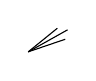
\begin{tikzpicture}\draw (0,0)--(.5,.28);\draw (0,0)--(.47,.16);\draw (0,0)--(.37,.30);\end{tikzpicture}}
\[
x\in\uline{X\supset K\supset S}\qquad\uline{p},\uline{q}
\]

\diagram{\begin{tikzcd}[ampersand replacement=\&,column sep=large]
\&\Gamma_{\infty\infty}\supset\Pi\arrow[dl]\arrow[d]\\
\Gamma_{\infty,3}\&\Gamma_{p,q}\supset\Pi
\end{tikzcd}}

\figure{\begin{tikzpicture}[x=.8cm,y=.8cm]
\draw (0,6)--(5.1,6)..controls(5.1,5.4)and(5.05,5)..(5.2,4.65);
\draw (5.05,4.5)--(11.5,4.5);
\draw (9.05,4.5)..controls(9.4,5.6)and(9.6,7.3)..(10.1,7.3);
\draw[line width=1.4pt] (9.05,4.5)--(9.4,4.35);
\node at (10.7,6.8) {$V\ni e$};
\node at (10.6,5.95) {$\uuline{\omega_1},\uuline{\omega_2}$};
\node at (10.65,5.15) {$\unsure{\mathrm I}(\omega_2/\omega_1)>0$};
\node at (2.3,5.65) {$C_{\infty,3}$};
\draw[->,thick] (2.3,5.25)--(2.3,2.6);
\draw (2.5,2.55)..controls(3.7,2.5)and(3.7,1.1)..(3.2,.7);
\draw (2.3,2.55)..controls(.7,2.1)and(1.1,.4)..(2.6,.45);
\draw (1.4,1.3)..controls(2,.95)and(2.9,.9)..(3.4,1.3);
\draw[dashed] (1.4,1.3)..controls(1.65,1.9)and(3,1.85)..(3.4,1.3);
\fill (1.85,1.14) circle(.065);\fill (3,1.13) circle(.065);\fill (2.55,1.69) circle(.065);
\node at (7,3.95) {$\Gamma_{21}$};
\draw (8.9,3.45)..controls(8,3.55)and(7.7,2.7)..(7.8,2.4);
\draw (8.9,3.45)..controls(9.8,3.7)and(10.1,3.3)..(10,2.8);
\draw (7.8,2.7)..controls(8,1.7)and(8.8,1.7)..(9.8,2.6);
\draw (7.8,2.7)..controls(8.7,3.2)and(9.7,3.1)..(9.8,2.6);
\draw (7.8,2.4)..controls(7.75,1.3)and(8.2,1.1)..(8.65,.95);
\draw (10,3)..controls(10.05,1.4)and(9.7,1.05)..(9.1,.9);
\draw (7.8,2.7)--(9.75,3.35)--(7.75,1.9)--(9.85,2.65)--(8.45,1.4)..controls(8.2,1.1)and(9.4,1.6)..(9.85,1.6);
\fill (8.95,3.45) circle(.065);\fill (9.1,1.98) circle(.065);\fill (9.05,.95) circle(.065);
\node at (11.1,3.65) {$\omega_1,\omega_2$};
\node at (11.2,2.85) {$\omega_2/\omega_1=\tau$};
\node at (5,4.05) {$\unsure{1}$};
\node[anchor=north] at (5.8,3.55) {\diagram{\begin{tikzcd}[ampersand replacement=\&,row sep=small]
\Pi_1\arrow[d]\\
\Gamma^{\circ}_{\infty,3}=\operatorname{SL}(\unsure{7|2},\mathbf Z)/(\pm1)\arrow[d]\\
\mathfrak S_3\arrow[d]\\1
\end{tikzcd}}};
\end{tikzpicture}}

\diagram{\begin{tikzcd}[ampersand replacement=\&,row sep=small]
\{\sigma_0,\sigma_1,\sigma_\infty\mid\overline{\rho_{\unsure{\delta}}^{3}=1}\arrow[d,equal]\\
\Gamma_{\infty3}\supset\Pi\arrow[d,rightsquigarrow]\\
\rho_{\unsure{\delta}}\qquad\uline{\rho_{\unsure{\delta}}^p}
\end{tikzcd}}

\figure{\begin{tikzpicture}
\draw[gray] (.5,2.7)--(1.4,2.7);\fill (.5,2.7) circle(.02);\fill (1.4,2.7) circle(.02);
\draw[->] (1.1,0.6)..controls(-.4,.6)and(-.5,2.1)..(.8,2.4)..controls(2.8,2.9)and(2.6,.6)..(1.1,.6);
\draw[dashed] (-.1,1.8)--(-.1,.85);
\node at (.35,1.7) {$\times$};\node at (.4,1.38) {$0$};
\node at (.9,1.7) {$\times$};\node at (1.15,1.33) {$\unsure{2^3.34}$};
\fill (2,1.65) circle(.045);
\node at (2.8,1.5) {$C_{11}$};
\node at (1,.25) {$R\ \unsure{\text{quot}(p,q)}$};
\draw[->] (.1,0)--(.1,-.6);
\node[anchor=north] at (.1,-.7) {\diagram{\begin{tikzcd}[ampersand replacement=\&,row sep=large]
\Gamma_{p,q}\arrow[d]\\\Gamma_{p',q'}
\end{tikzcd}}};
\end{tikzpicture}}

\diagram{\begin{tikzcd}[ampersand replacement=\&,row sep=large]
C_{\infty3}\arrow[d]\\C_{p3}
\end{tikzcd}}

\diagram{\begin{tikzcd}[ampersand replacement=\&,row sep=large]
C_{pq}\arrow[d]\\C_{p',q'}\arrow[d,equal]\\C_{pq}/R
\end{tikzcd}}
\[
\begin{gathered}p'\mid p\\q'\mid q.\end{gathered}
\qquad
\begin{array}{cc}C_{21}&C_{12}\\&C_{11}\end{array}
\]

\mspage{9}

\scanpage{11}
Carte trouée
\diagram{\begin{tikzcd}[ampersand replacement=\&,column sep=small]
(X\arrow[d]\supset K\arrow[dr])\&\&\text{tels que}\\
\text{surf. top.}\&\begin{gathered}\text{sous-variété fermée}\\\text{de dim 1}\end{gathered}\&
\end{tikzcd}}

\unsure{tte} comp. de $\operatorname{Déc}(X,K)$ est homéomorphe à un $D_n^*$

(disque troué \unsure{standart}, $1\leq n\leq+\infty$)

$\Pi_n$ pol. comb. \unsure{ép.} d'ordre $n$
\[
\uline{|\Pi_n|\times]0,1]}\supset|\Pi_n|\supset S_n
\qquad
\begin{gathered}\Pi_n:(S_n,A_n,R_n)\\S_n\subset|\Pi_n|\end{gathered}
\]
\[
D_n^*=|\Pi_n|\times]0,1]\setminus S_n
\]

\figure{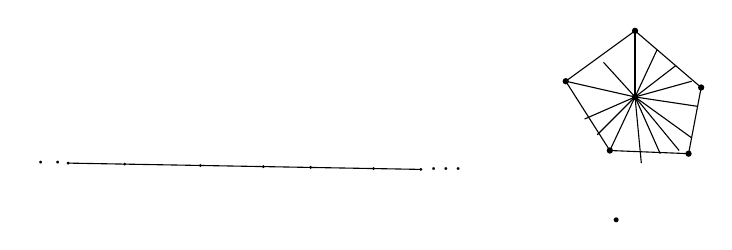
\begin{tikzpicture}[x=.8cm,y=.8cm]
\draw (9,3.1)--(10.05,2.2)--(9.85,1.15)--(8.6,1.2)--(7.9,2.3)--cycle;
\foreach \x/\y in {9/3.1,10.05/2.2,9.85/1.15,8.6/1.2,7.9/2.3,9/2.05}{\fill (\x,\y) circle(.05);}
\foreach \x/\y in {9/3.1,9.35/2.8,9.65/2.55,9.9/2.3,10/1.9,9.9/1.4,9.7/1.2,9.4/1.15,9.1/1.0,8.6/1.2,8.4/1.45,8.2/1.7,7.9/2.3,8.5/2.6}{\draw (9,2.05)--(\x,\y);}
\node at (-.3,1) {$\cdot\ \cdot$};
\draw (0,1)--(5.6,.9);
\foreach \x in {0,.9,2.1,3.1,3.85,4.85,5.6}{\fill (\x,{1-.1*\x/5.6}) circle(.025);}
\node at (6,.9) {$\ldots$};
\fill (8.7,.1) circle(.04);
\end{tikzpicture}}

\figure{\begin{tikzpicture}[x=.8cm,y=.8cm]
\draw[->] (3.4,6.2)--(1.3,5.55);
\draw[->] (2.55,5.75)--(2.2,6.35);
\draw[->] (3.8,6.2)..controls(4.5,5.95)and(5.3,6)..(5.9,5.65);
\draw[->] (4.55,5.85)--(4.7,6.3);
\draw[->,thick] (6.2,5.35)--(7.15,4.05);
\draw (7.1,4.25)..controls(7.4,3.9)and(7.5,3.6)..(7.45,3.5);
\draw (3.4,5.9)--(1.7,3);
\draw (5.15,4.9)--(5,4.4);\draw (4.9,4.2)--(3.65,2.1);
\draw (7.1,3.4)..controls(7,2.8)and(6.8,2.3)..(6.5,1.9);
\draw (7.6,3.3)..controls(7.85,2.3)and(7.5,1.8)..(7.65,1.2);
\node at (3.5,.8) {$E$};
\node at (1,.65) {$\uline{\sigma_0\ \sigma_1}\ \sigma_2$};
\draw (9.6,5.45) ellipse (1.02 and .94);
\draw (10.65,6.9)--(10.65,3.1);
\draw[thick] (9.6,5.45)--(10.65,5.4);
\draw (8.8,4.85)--(10.75,6.25);
\draw (8.8,4.85)--(8.91,5.03)--(8.96,4.86)--(9.03,5.14)--(9.09,4.98)--(9.16,5.22)--(9.22,5.07)--(9.29,5.31)--(9.35,5.18)--(9.48,5.4);
\foreach \x/\y in {9.45/6.38,8.65/5.75,8.8/4.85,9.82/4.51,10.63/5.16,10.65/5.4,10.42/6.0,9.6/5.45}{\fill (\x,\y) circle(.045);}
\draw[->,thick] (9.4,4.53)--(9,4.62);
\node at (11.65,5.7) {$\pm\frac1n$};
\draw (9.45,1.95) ellipse (1.15 and 1.1);
\draw[line width=2pt] (9.25,3.04) arc[start angle=100,end angle=38,x radius=1.15,y radius=1.1];
\draw[line width=2pt] (10.52,1.58)--(10.35,1.19);
\draw[line width=2pt] (10.05,1.02)..controls(9.9,.8)and(9.65,.81)..(9.4,.82);
\draw[line width=2pt] (8.31,2.25)--(8.31,1.55);
\draw[->,thick] (8.65,2.8)--(8.32,2.57);
\draw (8.3,2.52)--(8.45,2.32);\draw (8.19,2.2)--(8.43,2.22);
\draw[->] (9.4,1.4)..controls(10,1.6)and(10,1.9)..(9.9,2.2);
\draw[dashed] (12.65,1.48) circle(.25);
\draw[gray,densely dotted] (12.9,.65) circle(.3);
\draw (13.1,-.15) circle(.17);\draw[gray] (13.12,-.13) circle(.17);
\end{tikzpicture}}

\figure{\begin{tikzpicture}
\node[draw,inner sep=8pt] at (5,3.5) {$\operatorname{Déc}(\hat X,\unsure{\omega|W})$};
\node at (8.4,3.4) {$\tilde X-F$};
\draw (2.1,3.55)--(2.4,3.2)--(3.8,2.55)--(3.5,.9)--(2,{.2+1})--(1.65,2.65)--cycle;
\draw (2.1,3.55)--(1.85,4.1);\draw (2.1,3.55)--(2.4,3.95);
\draw (1.65,2.65)--(.6,2.75);\draw (1.65,2.65)--(1.55,3.3)--(2.1,3.55);
\draw (2.4,3.2)--(1.65,2.65);
\draw (3.8,2.55)--(4.5,3);\draw (3.5,.9)--(3.8,.5);\draw (2,1.2)--(1.7,.5);
\foreach \x/\y in {2.4/3.2,3.8/2.55,3.5/.9,2/1.2,1.65/2.65}{\fill (\x,\y) circle(.04);\draw (\x,\y) circle(.19);}
\draw (2.7,2.1) circle(.15);\fill (2.7,2.1) circle(.035);
\draw (5.3,2)--(5.8,2.45);\draw (5.3,2)--(5.25,2.45);\draw (5.3,2)--(4.95,2.2);\draw (5.3,2)--(4.9,1.65);\draw (5.3,2)--(5.4,1.65);\draw (5.3,2)--(5.85,1.95);
\end{tikzpicture}}

\mspage{10}

\scanpage{12}
\[
n\left\{\begin{array}{ll}L&d\text{ gén.}\\\cup&\\L'&d'\text{ gén}\end{array}\right.
\qquad\begin{gathered}(d'-1)=n(d-1)\\2=2.1\end{gathered}
\qquad\textcircled{1}
\]

\figure{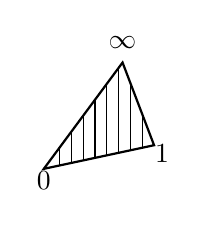
\begin{tikzpicture}
\draw[thick] (0,0)--(1,1.35)--(1.4,.3)--cycle;
\foreach \x in {.2,.35,.5,.65,.8,.95,1.1,1.25}{\draw (\x,{.214*\x})--(\x,{min(1.35*\x,3.975-2.625*\x)});}
\node at (0,-.15) {$0$};\node at (1.5,.2) {$1$};\node at (1,1.6) {$\infty$};
\end{tikzpicture}}

\figure{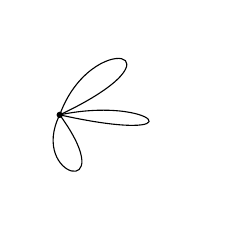
\begin{tikzpicture}
\draw (0,0)..controls(.4,1.1)and(1.7,.8)..(0,0);
\draw (0,0)..controls(1.2,.25)and(1.8,-.4)..(0,0);
\draw (0,0)..controls(-.4,-.8)and(.8,-1.1)..(0,0);
\fill (0,0) circle(.04);
\end{tikzpicture}}

\[
\begin{array}{lll}L\simeq\pi_1(X)&&1-d\\\cup&&\\L'\simeq\pi_1(X')&&1-d'\end{array}
\]
\[
\pi^+
\]
\diagram{\begin{tikzcd}[ampersand replacement=\&,column sep=small,row sep=small]
\rho_0\arrow[d]\&\rho_1\arrow[dd]\&\rho_\infty\arrow[d]\\
\rho_0^{-1}.\&\&\rho_\infty^{-1}\\
\&\rho_\infty\rho_0\&
\end{tikzcd}}

\[
\pi
\]
\diagram{\begin{tikzcd}[ampersand replacement=\&,column sep=large,row sep=large]
\&\&\margin{\text{avec }\varinjlim}\\
\operatorname{Ens}(\pi)\arrow[r,"\begin{gathered}F\\\text{commutant}\end{gathered}","\text{aux }\varinjlim"']\arrow[d,leftrightarrow]\&C\arrow[r,bend right=12,"G\text{ commute}","\text{aux }\varinjlim"']\arrow[ur,bend left=15]\&C'\\
\phantom{X}\&X\quad\pi\text{-objet }\inserted{\text{à droite}}\text{ de }C\&
\end{tikzcd}}
\margin{$(\simeq\operatorname{Ens}/\pi))$}

\[
F\longmapsto F(\underline{\pi_s})
\]
\[
X\longmapsto F_X:E\longmapsto\underbrace{X\times_\pi E}_{\in\operatorname{Ob}C}
\]
\[
\operatorname{Hom}_C\bigl(X\times_\pi E,
\underset{\substack{\rotatebox{90}{\ensuremath{\in}}\\\operatorname{Ob}C}}{\deleted{E}\inserted{\unsure{Y}}}\bigr)
\simeq\operatorname{Hom}_\pi\bigl(E,\operatorname{Hom}(X,Y)\bigr)
\]
\[
E\simeq\coprod_{i\in I}\pi/H_i
\]
\[
X\times_\pi E=\coprod_i\underbrace{X\times_\pi(\pi_s/H_i)}_{X/H_i}
\]

\mspage{11}

\scanpage{13}
\uline{Ex} $C=\operatorname{Ens}(\pi')$
\margin{\textcircled{2}}

\diagram{\begin{tikzcd}[ampersand replacement=\&,row sep=large]
\underline{\operatorname{Hom}}_!\bigl(\operatorname{Ens}(\pi),\operatorname{Ens}(\pi')\bigr)\arrow[r,phantom,"\simeq"]\&{}_{\pi'}\operatorname{Ens}_\pi\arrow[d]\\
\&{}_{\pi'}X_\pi
\end{tikzcd}}
\margin{commutant aux $\varinjlim$}

\diagram{\begin{tikzcd}[ampersand replacement=\&,column sep=large]
X\arrow[d,leftrightarrow]\&\operatorname{Ens}(\pi)\arrow[d]\\
F:\&E\arrow[r,maps to]\&X\times_\pi E
\end{tikzcd}}

\uline{Proposition} Pour que $F$ soit exact à gauche,
il f. et s. que $X$ soit un $\pi$-torseur à droite.
\figure{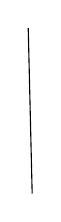
\begin{tikzpicture}\draw (0,0)--(.05,-2.1);\end{tikzpicture}}

$X$ torseur sous $\pi$
\[
{}^X\pi\overset{\mathrm{df}}=X\times_\pi\operatorname{int}(\pi)=\operatorname{Aut}_\pi(X)
\]
\[
\pi'\longrightarrow\operatorname{Aut}_\pi(X)
\]

\uline{Corollaire} Pour que $F$ soit équivalence, il f. et s. que
$\pi'\xrightarrow{\sim}\operatorname{Aut}_\pi(X)$, i.e. que $X$ soit un
bitorseur sous $\pi',\pi$; donc

\diagram{\begin{tikzcd}[ampersand replacement=\&,column sep=large,row sep=large]
\underline{\operatorname{Équiv}}\bigl(\operatorname{Ens}(\pi),\operatorname{Ens}(\pi')\bigr)\arrow[r,phantom,"\approxeq"]\arrow[d,"\unsure{\wr|u}"',"u\longmapsto u^{[-1]}"]\&\unsure{\operatorname{BiL}|\operatorname{BiT}}(\pi',\pi^{\unsure{3|*}})\arrow[d,"\unsure{\wr|u}"]\\
\underline{\operatorname{Équiv}}\bigl(\operatorname{Ens}(\pi'),\operatorname{Ens}(\pi)\bigr)\arrow[r,"\approx"]\&\operatorname{BiT}(\pi,\pi')
\end{tikzcd}}

\mspage{12}

\scanpage{14}
\deleted{\uline{\unsure{Bitinvol}}}
\[
{}_\pi X_\pi\qquad X\circ X\overset{\mu}{\xleftarrow{\sim}}1
\]
\[
\lambda e=e\lambda\qquad\forall\lambda\in\pi
\]
\[
\underline{\operatorname{Bitinvol}}(\pi)\xrightarrow{\approx}
\underline{\operatorname{Invol}}\bigl(\operatorname{Ens}(\pi)\bigr)
\]
\[
\xrightarrow{\approx}\underline{\operatorname{Ext}}(\mathbf Z/2,\pi)
\]

\deleted{$\unsure{E}\longleftarrow\unsure{1}.$}
\diagram{\begin{tikzcd}[ampersand replacement=\&,column sep=small]
1\arrow[r]\&\pi\arrow[r]\&\tilde\pi\arrow[r,"p"]\&\unsure{\mathbf Z/2}\arrow[r]\&1
\end{tikzcd}}
\diagram{\begin{tikzcd}[ampersand replacement=\&,column sep=small]
p^{-1}(1)\arrow[dr,bend right]\&\\
\&\text{él. non neutre}
\end{tikzcd}}

\figure{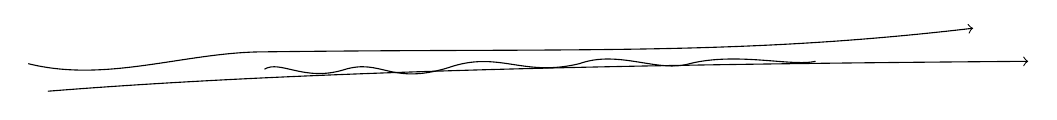
\begin{tikzpicture}
\draw[->] (0,.2)..controls(1,-.05)and(2,.35)..(3,.35)..controls(7,.4)and(9,.3)..(12,.65);
\draw[->] (.25,-.15)..controls(4,.15)and(9,.2)..(12.7,.23);
\draw (3,.13)..controls(3.2,.25)and(3.5,-.03)..(4,.12)..controls(4.5,.28)and(4.6,-.1)..(5.4,.17)..controls(6,.35)and(6.3,.03)..(7,.2)..controls(7.5,.38)and(8,.08)..(8.4,.2)..controls(9,.35)and(9.7,.16)..(10,.23);
\end{tikzpicture}}

$I$ \deleted{\illegible{1}} pol. comb. fini d'ordre $n\geq3$

``carte $n$-gonale $I$-\unsure{pondérée}

$u\in D_I$

\deleted{\[
\Pi_I=\frac{\underset{\substack{\downarrow\\\unsure{\text{libre}}\\\unsure{\text{eng. par }}I}}{L_I}}
{(\unsure{\lambda_0}\,\unsure{\lambda_i},\ \unsure{\lambda_{n-1}^{2}}=1)}
\qquad\unsure{I}\ \unsure{\text{n'est}}
\]}

\[
\Pi_I=\deleted{\unsure{L_I}}(\mathbf Z/2)^{*I}
\]
\deleted{\[
\unsure{\lambda_0}\,\underset{\unsure{n-1}}{\unsure{\lambda_i}}\,
\lambda_0\lambda_{n-1}\lambda_{\unsure{n-2}}\ldots\lambda_1=1
\]}

\diagram{\begin{tikzcd}[ampersand replacement=\&,column sep=small,row sep=large]
1\arrow[r]\&\Pi_I^+\arrow[r]\arrow[d,"\unsure{\wr|2}"']\&\Pi_I\arrow[r]\&\mathbf Z/2\arrow[r]\&1\\
\&\uline{L_I/\text{---}}\&\mathfrak S_I\&\&
\end{tikzcd}}

\figure{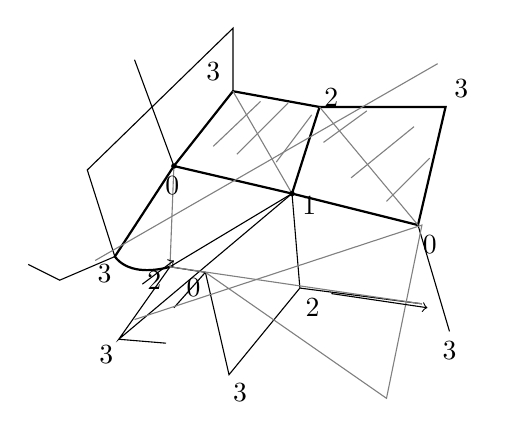
\begin{tikzpicture}[x=1cm,y=1cm]
\draw[thick] (1.2,3.3)--(1.95,4.25)--(3.05,4.05)--(2.7,2.95)--cycle;
\draw[thick] (3.05,4.05)--(4.65,4.05)--(4.3,2.55)--(2.7,2.95);
\draw (4.3,2.55)--(4.7,1.2);
\draw (2.7,2.95)--(2.8,1.75)--(4.35,1.55);
\draw (2.8,1.75)--(1.9,.65)--(1.6,1.95)--(1.15,2.02)--(2.7,2.95);
\draw[thick] (1.2,3.3)--(.45,2.15)..controls(.6,1.95)and(.9,1.95)..(1.15,2.02);
\draw (1.15,2.02)--(.5,1.1)--(2.7,2.95);
\draw (.5,1.1)--(1.1,1.05);
\draw (1.2,3.3)--(.7,4.65);
\draw (.45,2.15)--(.1,3.25)--(1.95,5.05)--(1.95,4.25);
\draw (.45,2.15)--(-.25,1.85)--(-.65,2.05);
\draw (1.6,1.95)--(1.2,1.5);
\draw[gray] (.2,2.1)--(4.55,4.6);
\draw[gray] (.7,1.35)--(4.35,2.55)--(3.9,.35)--(1.6,1.95);
\draw[gray] (1.2,3.3)--(1.15,2.02)--(4.35,1.55);
\draw[gray] (1.95,4.25)--(2.7,2.95);\draw[gray] (1.7,3.55)--(2.3,4.12);\draw[gray] (2.0,3.45)--(2.65,4.1);\draw[gray] (2.5,3.35)--(2.95,3.95);
\draw[gray] (3.05,4.05)--(4.3,2.55);\draw[gray] (3.1,3.6)--(3.65,4);\draw[gray] (3.45,3.15)--(4.25,3.8);\draw[gray] (3.9,2.85)--(4.45,3.4);
\fill (1.2,3.3) circle(.035);\fill (2.7,2.95) circle(.035);
\node at (1.18,3.05) {$0$};\node at (2.92,2.8) {$1$};\node at (3.2,4.17) {$2$};
\node at (1.7,4.5) {$3$};\node at (4.85,4.28) {$3$};\node at (4.45,2.3) {$0$};\node at (4.7,.95) {$3$};
\node at (2.96,1.5) {$2$};\node at (2.04,.42) {$3$};\node at (1.45,1.75) {$0$};\node at (.95,1.85) {$2$};\node at (.34,.9) {$3$};\node at (.32,1.93) {$3$};
\draw[->,thin] (.8,1.8)--(1.2,2.1);\draw[->,thin] (3.2,1.68)--(4.42,1.5);
\end{tikzpicture}}

\mspage{13}

\scanpage{15}
\figure{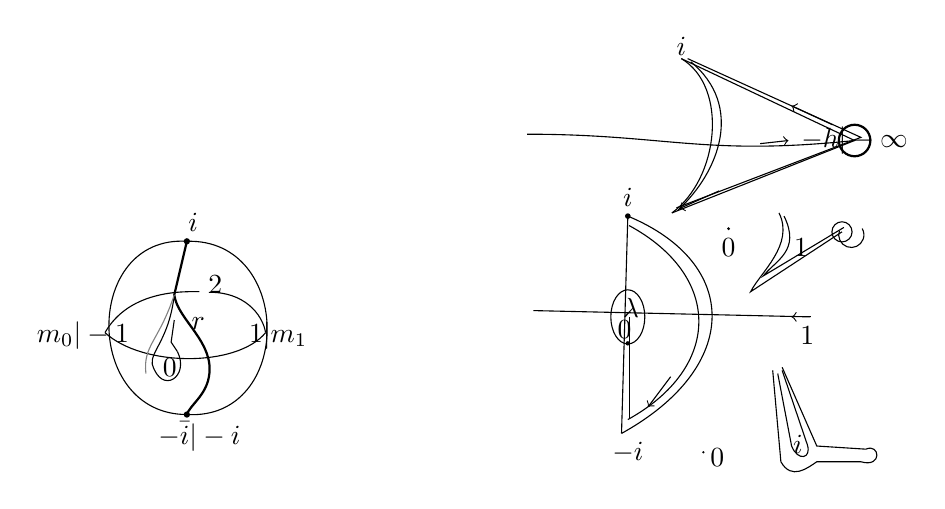
\begin{tikzpicture}[x=.8cm,y=.8cm]
\draw (1.8,3.65)..controls(.15,3.75)and(.15,.9)..(1.8,.9)..controls(3.5,.8)and(3.5,3.7)..(1.8,3.65);
\draw (.5,2.2)..controls(1.1,1.65)and(2.6,1.65)..(3.05,2.2);
\draw (.5,2.2)..controls(.9,2.9)and(1.8,2.85)..(2.0,2.85);
\draw (2.15,2.84)..controls(2.7,2.85)and(3,2.5)..(3.05,2.2);
\draw[thick] (1.8,3.65)--(1.6,2.8)..controls(1.65,2.4)and(2.25,2.05)..(2.15,1.5)..controls(2.1,1.2)and(1.85,1.05)..(1.8,.9);
\draw (1.6,2.8)..controls(1.52,2.1)and(1.22,1.9)..(1.25,1.7)..controls(1.4,1.2)and(1.85,1.5)..(1.65,1.9);
\draw (1.6,2.4)--(1.55,2.05)--(1.65,1.9);
\draw[gray] (1.6,2.8)..controls(1.35,2.05)and(1.1,2)..(1.15,1.55);
\fill (1.8,3.65) circle(.05);\fill (1.8,.9) circle(.05);
\node at (1.9,3.95) {$i$};\node at (2,.55) {$\unsure{-\bar i|-i}$};
\node at (.15,2.15) {$\unsure{m_0|-1}$};\node at (3.25,2.15) {$\unsure{1|m_1}$};
\node at (2.25,2.96) {$2$};\node at (1.53,1.65) {$0$};\node at (1.98,2.35) {$\unsure{r}$};
\draw (9.65,6.55)--(12.4,5.25)--(9.5,4.1);
\draw (9.75,6.55)--(12.5,5.3)--(9.57,4.18);
\draw (9.65,6.55)..controls(10.4,6.1)and(10.25,4.65)..(9.5,4.1);
\draw (9.8,6.5)..controls(10.65,5.8)and(10.25,4.75)..(9.6,4.15);
\draw[->] (12.05,5.5)--(11.4,5.8);\draw[->] (10.25,4.45)--(9.62,4.17);
\draw (7.2,5.35)..controls(9.4,5.35)and(10,5)..(12.4,5.25);
\draw[->] (10.9,5.2)--(11.35,5.25);
\draw[thick] (12.4,5.25) circle(.25);\node at (12.4,5.25) {$\unsure{-h|-\infty}$};
\node at (9.65,6.75) {$\unsure{i}$};
\draw (8.8,4.05)--(8.7,.6);
\draw (8.8,4.05)..controls(10.6,3.3)and(10.6,1.65)..(8.7,.6);
\draw (8.82,3.9)..controls(10.3,3.1)and(10.3,1.65)..(8.8,.82);
\draw (8.82,2.45)--(8.82,.85);\draw[->] (9.48,1.5)--(9.12,1.02);
\draw (7.3,2.55)--(11.7,2.45);\draw[->] (11.7,2.45)--(11.4,2.45);
\draw (8.8,2.45) ellipse (.27 and .43);
\node at (8.85,2.6) {$\unsure{\lambda}$};\node at (8.75,2.25) {$0$};
\node at (8.8,4.35) {$i$};\node at (8.8,.3) {$-i$};\node at (11.65,2.15) {$1$};
\fill (8.8,4.05) circle(.045);\fill (8.8,2.03) circle(.035);
\node at (10.4,3.55) {$0$};\fill (10.4,3.85) circle(.025);
\draw (11.2,4.1)..controls(11.45,3.6)and(10.9,3.15)..(10.75,2.85)--(12.2,3.8);
\draw (11.28,4.05)..controls(11.55,3.5)and(11.15,3.35)..(10.95,3.1)--(12.23,3.87);
\draw (12.2,3.8) circle(.16);\draw (12.16,3.82) arc[start angle=160,end angle=390,radius=.2];
\node at (11.55,3.55) {$\unsure{1}$};
\draw (11.1,1.6)--(11.23,.15)..controls(11.4,-.15)and(11.65,.05)..(11.8,.15)--(12.5,.15)..controls(12.85,.05)and(12.8,.45)..(12.58,.35)--(11.8,.4)--(11.25,1.65);
\draw (11.18,1.55)--(11.4,.4)..controls(11.5,.15)and(11.72,.2)..(11.65,.42)--(11.25,1.6);
\node at (11.5,.42) {$\unsure{i}$};
\fill (10,.3) circle(.02);\node at (10.22,.21) {$0$};
\end{tikzpicture}}

\[
\pi\qquad\lambda_0\ \lambda_1\ \lambda_2\ \lambda_3\qquad\varepsilon
\]
\deleted{\[
\lambda_0\lambda_1\lambda_2\lambda_3=1
\]}
\deleted{\[
\lambda_3\lambda_2\lambda_1\lambda_0=1
\]}
\[
\varepsilon^2=1\qquad
\begin{cases}\varepsilon\lambda_0\varepsilon^{-1}=\lambda_0^{-1}\\
\varepsilon\lambda_1\varepsilon^{-1}=\lambda_{\unsure{1}}^{-1}
\end{cases}
\qquad\varepsilon\lambda_i\varepsilon^{-1}
\]
\[
\operatorname{Hom}(i,-i)
\]
\diagram{\begin{tikzcd}[ampersand replacement=\&,column sep=large,row sep=small]
\operatorname{Hom}(-i,-i)\arrow[d,phantom,"\wr"]\&\operatorname{Hom}(i,i)\arrow[d,phantom,"\wr"]\\
\pi\&\pi
\end{tikzcd}}
\[
\ell\circ\bar\ell\qquad\lambda_1^{-1}\lambda_2^{-1}\lambda_1
\]
\diagram{\begin{tikzcd}[ampersand replacement=\&,column sep=large]
i\arrow[r,"\varepsilon^{-1}"]\&\unsure{\bar i|-i}\&\unsure{\bar i|-i}\arrow[r,"\overset{\longleftarrow}{\lambda_i}"]\&\unsure{\bar i|-i}\&\unsure{\bar i|-i}\arrow[r,"\varepsilon"]\&i
\end{tikzcd}}
\[
\varepsilon\circ\bar\lambda_i\circ\varepsilon^{-1}.
\]

\figure{\begin{tikzpicture}\fill (0,0) circle(.025);\end{tikzpicture}}
\diagram{\begin{tikzcd}[ampersand replacement=\&,row sep=small]
X\arrow[d]\&\Gamma\\\unsure{a}\&
\end{tikzcd}}
\[
(\gamma\in\Gamma,\ell\in\operatorname{Hom}(\gamma a,\deleted{\unsure{\gamma}}b))
\]
\[
(\gamma'\in\Gamma,\ell'\in\operatorname{Hom}(\gamma'b,\deleted{\unsure{\gamma'}}c))
\]
\[
\pi_1(X,\Gamma;a)\mathbin{-}\Gamma
\]

\diagram{\begin{tikzcd}[ampersand replacement=\&,column sep=large,row sep=large]
\gamma a\arrow[r,"\ell"]\&\deleted{\unsure{\gamma}}b\&\deleted{\unsure{\gamma'a\ \gamma'\ell}}:\\
\&\gamma'b\arrow[r,"\ell'"]\&\deleted{\unsure{\gamma'}}c
\end{tikzcd}}
\deleted{\diagram{\begin{tikzcd}[ampersand replacement=\&,column sep=large]
\unsure{\gamma b}\arrow[r,"\unsure{\gamma\ell'}"]\&\unsure{\gamma\gamma'c}
\end{tikzcd}}}

\diagram{\begin{tikzcd}[ampersand replacement=\&,column sep=large]
\gamma'\gamma a\arrow[r,"\gamma'(\ell)"]\&\gamma'b\arrow[r,"\ell'"]\&c
\end{tikzcd}}

\diagram{\begin{tikzcd}[ampersand replacement=\&,column sep=large]
a\arrow[r,dash,"(\gamma\ell')\circ\ell"]\&\gamma\gamma'c
\end{tikzcd}}
\[
(\gamma\gamma',(\gamma\ell')\circ\ell)
\]

\figure{\begin{tikzpicture}
\draw (0,.5)--(-.12,-2.8);
\node at (.7,.2) {$\gamma a$};\fill (1.75,.2) circle(.03);
\node at (.7,-.6) {$-\gamma'a$};\draw (1.35,-.6)--(1.8,-.6);\fill (2.05,-.6) circle(.03);
\end{tikzpicture}}

\[
(\gamma',\ell')\bigl(\gamma^{\deleted{\unsure{\prime}}},\ell^{\deleted{\unsure{\prime}}}\bigr)
=\Bigl(\gamma'\gamma^{\deleted{\unsure{\prime}}},
\deleted{(\unsure{\gamma}\ell')\circ\ell}\inserted{\ell'\circ\gamma'(\ell)}\Bigr)
\]
\figure{\begin{tikzpicture}\draw[thick] (0,0)--(.22,0);\end{tikzpicture}}

\mspage{14}

\scanpage{16}
\diagram{\begin{tikzcd}[ampersand replacement=\&,column sep=large]
\operatorname{Ens}(\pi)\arrow[r,"F_X","{}_{\pi'}X_\pi"']\&\operatorname{Ens}(\pi')\arrow[r,"F_Y","{}_{\pi''}Y_{\pi'}"']\&\operatorname{Ens}(\pi'')
%
\end{tikzcd}}
\[
F_Y\circ F_X=F_{Y\wedge_{\pi'}X}
\]
\figure{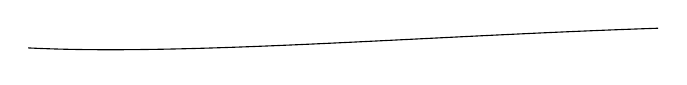
\begin{tikzpicture}\draw (0,0)..controls(2,-.1)and(5,.15)..(8,.25);\end{tikzpicture}}

${}_{\pi'}X_\pi$ bitorseur; \unsure{classifier} à isom près ?

\[
\pi'\xrightarrow{\sim}{}^X\pi
\overset{\substack{\text{non can.}\\\text{mais can. dans }\operatorname{Isomext}({}^X\pi,\pi)}}{\simeq}\pi
\]

Donc $X$ définit $\operatorname{Isomext}(\pi',\pi)$

\deleted{\unsure{Cl d'i.} de bit $(\pi',\pi)$}
\[
\pi_0\bigl(\underline{\operatorname{Bit}}(\pi',\pi)\bigr)
\xrightarrow{\sim}\operatorname{Isomext}(\pi',\pi)
\]

\diagram{\begin{tikzcd}[ampersand replacement=\&,column sep=large,row sep=huge]
\pi_0\bigl(\underline{\unsure{\operatorname{Bitpt}}}(\pi',\pi)\bigr)\arrow[r,phantom,"\simeq"]\arrow[d]\&\operatorname{Isom}(\pi',\pi)\arrow[dl,"\begin{gathered}\unsure{\text{surj.}}\\\unsure{\text{passage au quotient}}\\\text{par }\operatorname{Int}(\pi)\end{gathered}"]\\
\pi_0\bigl(\underline{\operatorname{Bit}}(\pi',\pi)\bigr)\simeq\operatorname{Isom}(\pi',\pi)/\operatorname{Int}(\pi)=\operatorname{Isomext}(\pi',\pi)\&
\end{tikzcd}}

\figure{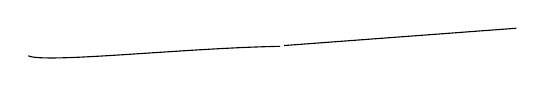
\begin{tikzpicture}\draw (0,0)..controls(.2,-.1)and(2,.1)..(3.2,.12);\draw (3.25,.13)--(6.2,.35);\end{tikzpicture}}

\diagram{\begin{tikzcd}[ampersand replacement=\&,column sep=large]
F^2\arrow[r,"\sim","\mu"']\&\operatorname{id}
\end{tikzcd}}
\diagram{\begin{tikzcd}[ampersand replacement=\&,column sep=large]
F(F(E))\arrow[r,"\mu_E"]\&E
\end{tikzcd}}
\diagram{\begin{tikzcd}[ampersand replacement=\&,column sep=large]
F(F(\underline{F(E)}))\arrow[r,shift left=2,"F(\mu_E)"]\arrow[r,shift right=2,"\mu_{F(E)}"']\&F(E)
\end{tikzcd}}
\[
\unsure{F\mu|F\circ\mu}=\mu\mathbin{\unsure{\cdot|\star}}F:F^3\longrightarrow F
\]

\mspage{15}

